\documentclass{report}
\usepackage[numbered, framed]{mcode}
% Langue
\usepackage[utf8]{inputenc}
\usepackage[T1]{fontenc}      
\usepackage[francais]{babel}
% Mise en forme générale
\usepackage[top=2.5cm,bottom=2.5cm,right=2.5cm,left=2.5cm]{geometry}
% Package divers
\usepackage{chemist} 
\usepackage[version=3]{mhchem}
\usepackage{chemfig}
\usepackage[squaren, Gray]{SIunits}
\usepackage{sistyle}
\usepackage[autolanguage]{numprint}
\usepackage{url}
\usepackage{rotating}
\usepackage{xcolor,colortbl}
\definecolor{Gray}{gray}{0.85}
% HEADER
\usepackage{fancyhdr}
\setlength{\headheight}{15.2pt}
\pagestyle{fancy}
\lhead[P3]{P3}
\chead[2014]{2014}
\rhead[gr1243]{gr1243}
\usepackage{hyperref}
\hypersetup{
    colorlinks,
    citecolor=black,
    filecolor=black,
    linkcolor=black,
    urlcolor=black
}
% Nouvelles commandes
\newcommand{\std}{\ensuremath{^{\circ}}}
\newcommand\ph{\ensuremath{\mathrm{pH}}}
\newcommand{\annexe}{\section{Annexes}}
\newcommand{\biblio}[1]{}
\newcommand{\doctitle}[1]{}
\title{Projet P3 - Rapport}
\author{\textbf{Groupe 124.3}\\
\textsc{Frenyo} Péter (6266-12-00)\\
\textsc{Gillain} Nathan (7879-12-00)\\
\textsc{Lamine} Guillaume (7109-13-00)\\
\textsc{Piraux} Pauline (2520-13-00)\\
\textsc{Paris} Antoine (3158-13-00)\\
\textsc{Quiriny} Simon (4235-13-00)\\
\textsc{Schrurs} Sébastien (7978-13-00)}
\date{\today}
\begin{document}
\maketitle
\tableofcontents

\chapter{Tache 1: Gestion des réactifs}
\documentclass{article}

\usepackage[utf8]{inputenc}
\usepackage[T1]{fontenc}      
\usepackage[francais]{babel}
\usepackage{chemist}
\usepackage{chemfig} 
\usepackage{lewis}
\usepackage[top=2.5cm,bottom=2.5cm,right=2.5cm,left=2.5cm]{geometry}
\usepackage[squaren, Gray]{SIunits}
\usepackage{url}
\usepackage{hyperref}
\hypersetup{
    colorlinks,
    citecolor=black,
    filecolor=black,
    linkcolor=black,
    urlcolor=black
}

\newcommand\chemfigc[1]{
\vspace{0.5cm}
\begin{center}\chemfig{#1}\end{center}
\vspace{0.5cm}}

\title{Projet 3 - Rapport de tâche 1}
\author{\textbf{Groupe 124.3}
\\
\textsc{Frenyo} P\'eter (6266-12-00)\\
\textsc{Gillain} Nathan (7879-12-00)\\
\textsc{Lamine} Guillaume (7109-13-00)\\
\textsc{Piraux} Pauline (2520-13-00)\\
\textsc{Paris} Antoine (3158-13-00)\\
\textsc{Quiriny} Simon (4235-13-00)\\
\textsc{Schrurs} Sébastien (7978-13-00)}
\date{\today} 
\begin{document}

\maketitle
\tableofcontents

\section{Calcul du flux des réactifs}

\paragraph{Hypothèse}
Lors du calcul de ces flux, nous avons utilisé l'hypothèse que tous les réactifs sont 
consommés par le réacteur.

\paragraph{Calculs}
L'équation de la réaction de production de l'ammoniac par le procédé \textsc{Haber-Bosch} est donnée par :

	\begin{chemmath}
			\frac{1}{2}N_2(g) + \frac{3}{2}H_2(g) \longrightarrow NH_3(g) + \Delta H
 	\end{chemmath}
	
En sachant que l'on cherche à produire \unit{1000}{\ton} de \chemform{NH_3} par jour, 
on calcule assez facilement le flux de \chemform{N_2} (les détails de calculs ont été omis
dans ce rapport)

	$$m_{N_2} = \unit{823.5}{\ton\per\dday}$$

et le flux de \chemform{H_2}

	$$m_{H_2} = \unit{176.4}{\ton\per\dday}.$$

\section{Calcul du débit d'eau nécessaire pour refroidir le réactif}
\paragraph{Hypothèses}
\begin{itemize}
	\item Les capacités calorifiques ne dépendent pas de la température ;
	\item La pression dans le réacteur est constante et vaut \unit{10^5}{\pascal}.
\end{itemize}

\paragraph{Première méthode : on considère les capacités calorifiques constantes}
Pour la réaction donnée dans la section précédente, on a $\Delta H(\unit{298.15}{\kelvin})
 = \unit{-46 \cdot 10^3}{\joule}$ pour une mole de \chemform{NH_3(g)} produite \cite{atkins}.
Comme la réaction a lieu à \unit{500}{\celsius} (c'est à dire \unit{773.15}{\kelvin}), il
va falloir calculer $\Delta H(\unit{773.15}{\kelvin})$. Pour cela, nous avons besoin
des capacités calorifiques moyenne à pression constante de chacun des réactifs et des produits
de la réaction. Nous trouvons ces données dans une table \cite{atkins}.

	$$
	\left\{
		\begin{array}{rl}
			C_{p_{NH_3(g)}} &= \unit{37}{\joule\per\mole\kelvin}\\
			C_{p_{H_2(g)}} 	&= \unit{28.836}{\joule\per\mole\kelvin}\\
			C_{p_{N_2(g)}} 	&= \unit{29.124}{\joule\per\mole\kelvin}
		\end{array}
	\right
	$$

On a donc :

$$\Delta H(\unit{773.15}{\kelvin}) = \Delta H(\unit{298.15}{\kelvin})
+ \int_{298.15}^{773.15} C_{p_{NH_3(g)}} dT - \frac{1}{2}\int_{298.15}^{773.15} C_{p_{N_2(g)}} dT
- \frac{3}{2} \int_{298.15}^{773.15} C_{p_{H_2(g)}} dT = \unit{-5.5887 \cdot 10^4}{\joule\per\mole}$$

Pour la quantité de \chemform{NH_3} à produire par jour (à savoir $\unit{58.83 \cdot 10^6}{\mole}$),
la quantité de chaleur produite est donc :

$$q = \Delta H(\unit{773.15}{\kelvin}) \cdot n_{NH_3} = \unit{-3.28786 \cdot 10^{12}}{\joule}$$

En connaissant la capacité calorifique de l'eau $C_{H_2O(g)} = \unit{4185.5}{\joule\per\kilo\gram\kelvin}$ \cite{atkins}et en égalant
$q$ à $m_{H_2O} \cdot C_{H_2O(g)} \cdot \Delta T$ avec $\Delta T = 90 - 25 = \unit{65}{\kelvin}$, on trouve un
flux d'eau égal à

$$m_{H_2O} = \unit{1.2085 \cdot 10^7}{\kilo\gram\per\dday} \Rightarrow V_{H_2O} \approx \unit{1.2085 \cdot 10^7}{\liter\per\dday} 
= \unit{139.8}{\liter\per\second}$$

\paragraph{Deuxième méthode : les capacités calorifiques dépendent de la température}
On peut être plus précis en utilisant les capacités calorifiques suivantes \cite{hc-table} :

	$$
	\left\{
		\begin{array}{rl}
			C_{p_{NH_3(g)}}(T) &= \unit{31.81 + (15.48 \cdot 10^{-3})T + (5.86 \cdot 10^{-6})T^2}{\joule\per\mole\kelvin}\\
			C_{p_{H_2(g)}}(T) 	&= \unit{29.30 - (0.84 \cdot 10^{-3})T + (2.09 \cdot 10^{-6})T^2}{\joule\per\mole\kelvin}\\
			C_{p_{N_2(g)}}(T) 	&= \unit{27.62 + (4.19 \cdot 10^{-3})T}{\joule\per\mole\kelvin}
		\end{array}
	\right
	$$

En refaisant le calcul ci-dessus en tenant compte de la variation des capacités calorifiques en fonction
de la température, nous obtenons un débit un peu inférieur de \unit{135.662}{\liter\per\second}. On remarque
que l'approximation faite ci-dessus n'est pas si mauvaise que ça. Nous vous épargons ici
les détails de calculs (que nous avons réalisé avec \textsc{Matlab}).

\section{Sources des réactifs}
	\subsection{Sources de diazote}
	\subsubsection{Procédé cryogénique}
	Ce procédé se base sur la séparation des différents constituants de l'air en fonction de leur température 
	d'ébullition (l'oxygène \chemform{O_2} se condense avant le diazote \chemform{N_2}).
	L'air est purifié jusqu'à liquéfaction et les différents constituants sont séparés dans une colonne de 
	rectification par distillation fractionnée. Cette méthode permet d'avoir du diazote \chemform{N_2} pur 
	à \numprint{99,99}\%. Cette méthode est efficace pour une consommation au-delà de $\unit{200}{\meter\cubed\per\hour}$ \cite{scf}. 

	\subsubsection{Perméation gazeuse}
	Ce procédé utilise les différentes vitesses d'effusion des molécules de gaz à travers une membrane. 
	L'\chemform{O_2}, \chemform{H_2O} et le \chemform{CO_2} s'effusent plus rapidement que le \chemform{N_2}.
	Cette méthode nous permet d'obtenir du \chemform{N_2} sec pur à \numprint{95-99}. Ce procédé s'utilise pour des 
	débits forts variables ($\unit{3-1000}{\meter\cubed\per\hour}$) \cite{scf}.

	\subsubsection{Méthode de Ramsay}
	
	\begin{chemmath}
			NaNO_2(aq) + NH_4Cl(aq) \longrightarrow NaCl(aq) + 2 H_2O(l) + N_2(g)
	\end{chemmath}
	
	On chauffe le mélange de \chemform{NaNO_2} et \chemform{NH_4Cl} pour obtenir le \chemform{N_2} sous forme gazeuse.
	Un désavantage de cette méthode par rapport aux 2 premières est qu'il faut acheter les réactifs. De plus, il faut utiliser de l'énergie pour chauffer la réaction \cite{wiki-n2}.

	\subsection{Sources de dihydrogène}
		\subsubsection{Vaporeformage de méthane}
		2 réactions sont utilisées pour ce procédé \cite{afhypac} :
		
		\begin{chemmath} 
			CH_4 + H_2O \longleftrightarrow CO + 3H_2
		\end{chemmath}
		
		\begin{chemmath}
			CO + H_2O \longleftrightarrow CO_2 + H_2
		\end{chemmath}
		
		L'équation bilan obtenue est la suivante :
		
		\begin{chemmath}
			CH_4 + 2H_2O \longleftrightarrow CO_2 + 4 H_2
		\end{chemmath}
		
			Cette réaction nécessite un catalyseur : le nickel. Le rendement varie entre $40-45\%$. Le problème de cette 
			méthode est qu'elle rejette une grande quantité de \chemform{CO_2}, gaz à effet de serre \cite{wiki-h2}.
			
		\subsubsection{Oxydation partielle d'hydrocarbure}
		\begin{chemmath}
			C_nH_m + \frac{n}{2} O_2 + \frac{3,76n}{2} N_2 \longrightarrow \frac{m}{2} H_2 + n CO + \frac{3,76n}{2} N_2
		\end{chemmath}
		L'air est comburant pour cette réaction, qui a besoin d'être catalysée. Son caractère exothermique aide à la catalyse. 
		L'inconvénient de cette méthode est son faible rendement \cite{wiki-h2}.

		\subsubsection{Electrolyse}
		Réaction à l'anode : 
		
		\begin{chemmath}
			2H_2O(l) \longrightarrow O_2(g) + 4 H^+(aq) + 4e^-
		\end{chemmath}
		
		Réaction à la cathode :
		
		\begin{chemmath}
			4H_2O(l) + 4e^- \longrightarrow 2H_2O(g) + 4OH^-(aq)
		\end{chemmath}
		
		L'équation bilan obtenue est la suivante :
		
		\begin{chemmath}
			2H_2O(l) \longrightarrow 2H_2(g) + O_2(g)
		\end{chemmath}
		
	La réaction nécessite une grande quantité d'électricité. L'eau, quant à elle, est présente en quantité illimitée 
	et est peu coûteuse. En pratique, cette méthode est très peu utilisée \cite{wiki-h2}.
	
	\section{Premier jet du flow-sheet simplifié}
	La première ébauche de notre flow-sheet se trouve à la figure \ref{flow-sheet}.
	
	\begin{figure}[htb!]
		\centering
		\rotatebox{90}{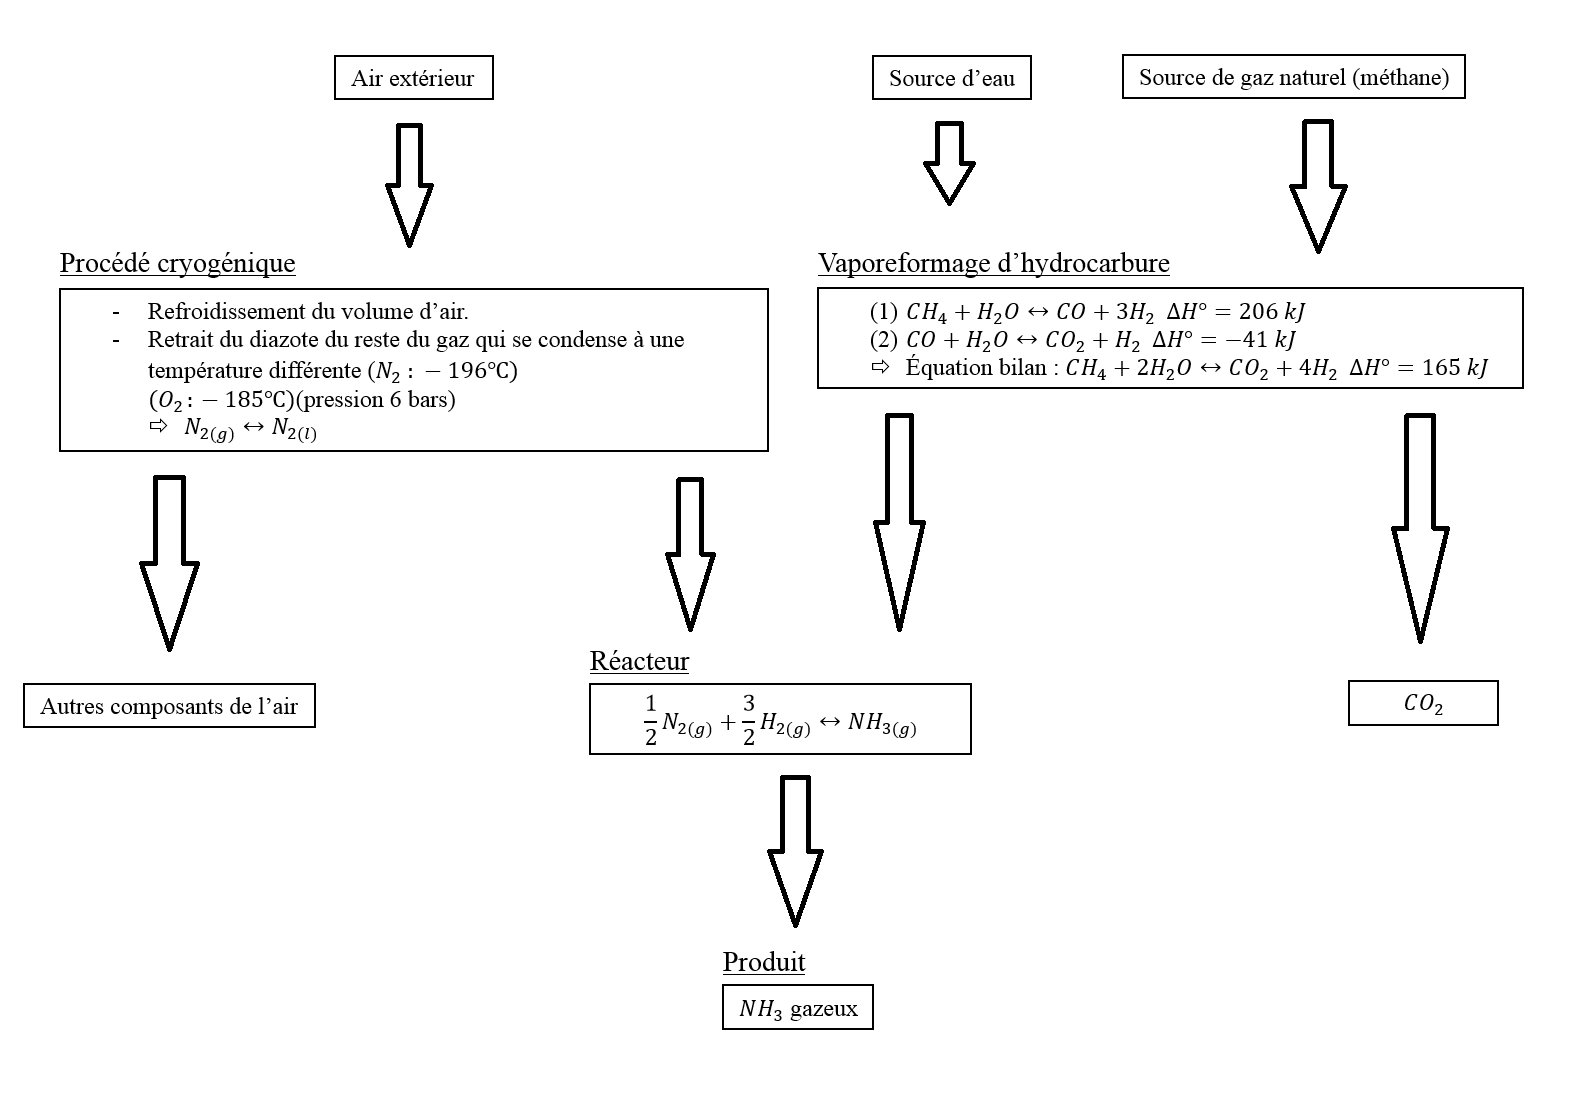
\includegraphics[scale=0.50]{flow-sheet.png}}
		\caption{Première ébauche de notre flow-sheet.}
		\label{flow-sheet}
	\end{figure}
	
	\section{Deuxième version du flow-sheet}
	Voici la deuxième version du flow-sheet (Figure \ref{flow-sheet-v2}).
	
	\begin{figure}[htb!]
	\centering
	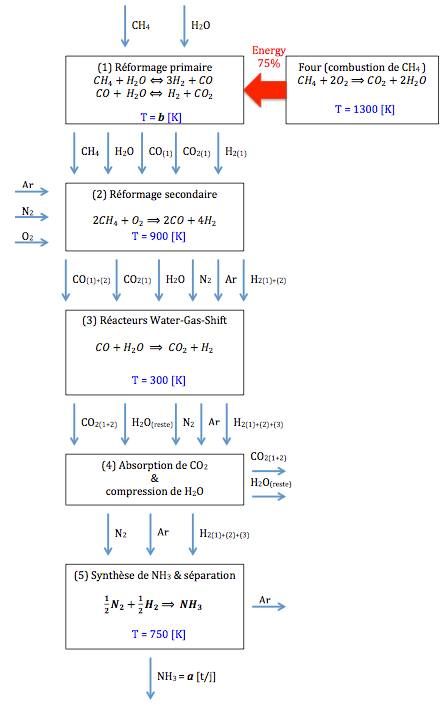
\includegraphics[scale=0.80]{flow-sheet-v2.jpg}
	\caption{Deuxième ébauche de notre flow-sheet.}
	\label{flow-sheet-v2}
	\end{figure}

\section{Bilan de matiere}
On pose le flux de \chemform{NH_3(g)} à la sortie égal à $\unit{m_{NH_3}}{\gram\per\dday}$. 

Nous partons de la réaction : 
\begin{chemmath}
		\frac{1}{2}N_2(g) + \frac{3}{2}H_2(g) \longrightarrow NH_3(g) 
\end{chemmath}
 	
$$m_{NH_3} = \unit{m_{NH_3}}{\gram\per\dday}$$ 

Et donc, 
 
$$n_{NH_3} = \unit{\frac{m_{NH_3}}{17}}{\mole}$$

Ce qui donne 

$$n_{N_2} = \frac{n_{NH_3}}{2} = \unit{\frac{m_{NH_3}}{34}}{\mole}$$ 

et 

$$n_{H_2} = \frac{3}{2} \cdot n_{NH_3}$$

On sait que le \chemform{N_2(g)} provient uniquement de l'air entrant 
dans le réacteur du  réformage primaire. Et comme on peut considérer
que l'air est composé de 78\% de \chemform{N_2(g)}, 21\% de \chemform{O_2(g)}
et 1\% d'\chemform{Ar(g)}, on peut déduire que $$n_{air}$$ entrant dans le 
réacteur du réformage primaire vaut : 

$$n_{air}= n_{N_2} \cdot \frac{100}{78} = \unit{\frac{25m_{NH_3}}{663}}{\mole}$$ 

Et :
$$n_{O_2}= n_{air} \cdot \frac{21}{100} = \unit{\frac{7m_{NH_3}}{884}}{\mole}$$
$$n_{Ar}= n_{air} \cdot \frac{1}{100} = \unit{\frac{1m_{NH_3}}{2652}}{\mole}$$

On sait par la réaction du réformage primaire suivante et par l'hypothèse que le
\chemform{CH_4(g)} et le \chemform{O_2(g)} sont présents en quantité stoechiométrique : 

\begin{chemmath}
	2CH_4 + O_2 \Longrightarrow 2CO + 4 H_2
\end{chemmath} 

que :

$$n_{CH_4} = 2 \cdot n_{O_2} = \unit{\frac{7m_{NH_3}}{442}}{\mole}$$
$$n_{CO} = n_{CH_4} =  \unit{\frac{7m_{NH_3}}{442}} {\mole}$$
$$n_{H_2} = 2 \cdot n_{CH_4} =  \unit{\frac{7m_{NH_3}}{221}}{\mole}$$

On s'intéresse ensuite à la réaction du Water-Gas-Shift : 

\begin{chemmath}
	CO + H_2O \Longrightarrow CO_2 + H_2
\end{chemmath} 

On sait que $n_{CO}$ du WGS = $n_{CO}$ produit au réformage primaire
$+ n_{CO}$ produit au réfomarge secondaire. 

Et donc on a : 

$$n_{CO_2} = n_{CO} = n_{H_2O}$$

S'il reste du \chemform{H_2O} à la fin de cette réaction, $n_{H2_O}$ 
sera égal à $n_{H2_O}$ du réformage primaire moins le $n_{CO}$ du WGS.

On peut aussi déduire que $n_{CO_2-tot} = n_{{CO_2}-\text{réformage primaire}}
+ n_{{CO_2}-\text{WGS}}$.

On peut aussi conclure que : 

$$n_{H_2-\text{réformage primaire}}= n_{H_2-\text{synthèse} \chemform{NH_3}}
- n_{H_2-\text{réformarge secondaire}} - n_{H_2-\text{WGS}}$$

% A transformer en tableau pour plus que ce soit plus clair.
Après la résolution de l'équilibre du réformage primaire, 
on obtient les valeurs suivantes : 

$$n_{H_2O-\text{réformage primaire}} = $$
$$n_{CO-\text{réformage primaire}} = $$
$$n_{CO_2-\text{réformage primaire}} = $$
$$n_{H_2-\text{réformage primaire}} = $$

$$n_{CO-\text{WGS}} = $$
$$n_{CO2-\text{WGS}} = $$
$$n_{H_2-\text{WGS}} = $$

$$n_{CO_2-\text{final}} = $$ 
$$n_{H_2O-\text{final}} = $$

\section{Equilibre du reformage primaire}
\subsection{Calcul de la constante d'équilibre}

Pour calculer la constante d'équilibre nous allons utiliser $K= \exp{\frac{-\Delta G}{RT}}$ avec $\Delta G = \Delta H - T \Delta S $

\subsubsection{Première équation}
\begin{chemmath} 
 CH_4(g) + H_{2}O(g) \longrightarrow CO(g) + 3H_2
\end{chemmath} 

Connaissant les capacités calorifiques dépendantes de la température:
$$
\left\{
	\begin{array}{rl}
		C_{p_{CO}}(T) 			&= \unit{27.62 +(5.02 \cdot 10^{-3})T}{\joule\per\mole\kelvin} \\
		C_{p_{H_{2}}}(T) 		&= \unit{29.3-(0.84 \cdot 10^{-3})T + (2.09\cdot 10^{-6})T^2}{\joule\per\mole\kelvin} \\
		C_{p_{CH_{4}}}(T) 	&= \unit{14.23+(75.3 \cdot 10^{-3})T - (18\cdot 10^{-6})T^2}{\joule\per\mole\kelvin} \\
		C_{p_{H_{2}O}}(T) 	&= \unit{30.13+(10.46 \cdot 10^{-3})T}{\joule\per\mole\kelvin} 
	\end{array}
\right
$$

$$
\Delta H_1(T) = \Delta H(\unit{298.15}{\kelvin}) 
 + \int_{298.15}^{T} C_{p_{CO(g)}} dT + 3\int_{298.15}^{T} C_{p_{H_2(g)}} dT 
 +  \int_{T}^{298.15} C_{p_{CH_4(g)}} dT + \int_{T}^{298.15}C_{p_{H_{2}O_{(g)}}}dT
 $$\\
  
 $$
 = 188369.87 + 71.16 T -0.04163 T^2 + (8.09\cdot 10^{-6}) T^3
 $$ 
 
 $$
 \Delta S_1(T) = \Delta S(\unit{298.15}{\kelvin}) 
 + \int_{298.15}^{T} C_{p_{CO(g)}} \dfrac{dT}{T} + 3\int_{298.15}^{T} C_{p_{H_2(g)}} \dfrac{dT}{T} 
 +  \int_{T}^{298.15} C_{p_{CH_4(g)}} \dfrac{dT}{T} + \int_{T}^{298.15}C_{p_{H_{2}O_{(g)}}}\dfrac{dT}{T}
 $$\\ 
 
 $$
 = -167.05 + 71.16 \ln T -0.08326 T + (1.2135\cdot 10^{-5} T^2
 $$ 
 
 $$
 \Delta G_1(T) = 188369.9 - (71.16\ln T)T + 238.21T + 0.04163 T^2 -(4.045\cdot 10^{-6}T^3
 $$ 

Nous obtenons donc
$$K_1 = \exp{\frac{-\Delta G_1}{RT}}$$
avec la valeur de $\Delta G_1$ calculée plus tôt.

\subsubsection{Deuxième équation}
\begin{chemmath} 
 CO(g) + H_{2}O(g) \longrightarrow CO_2(g) + H_2
\end{chemmath} 

Connaissant les capacités calorifiques dépendantes de la température de l'équation précedente et celle-ci:

$$
\begin{array}{rl}
C_{p_{CO_2}}(T)=32.22 +(22.18 \cdot 10^{-3})T + (3.35 \cdot 10^{-6})T^2\\
\end{array}
$$

$$
\Delta H_2(T) = \Delta H(\unit{298.15}{\kelvin}) 
 + \int_{298.15}^{T} C_{p_{CO_2(g)}} dT + \int_{298.15}^{T} C_{p_{H_2(g)}} dT 
 +  \int_{T}^{298.15} C_{p_{CO(g)}} dT + \int_{T}^{298.15}C_{p_{H_{2}O_{(g)}}}dT
 $$\\
  
 $$
 = -42533.33+3.77T+(2.93\cdot 10^-3)T^2-(4.2\cdot 10^-7)T^3
 $$ 

$$
\Delta S_2(T) = \Delta S(\unit{298.15}{\kelvin}) 
 + \int_{298.15}^{T} C_{p_{CO_2(g)}} \dfrac{dT}{T} + 3\int_{298.15}^{T} C_{p_{H_2(g)}} \dfrac{dT}{T} 
 +  \int_{T}^{298.15} C_{p_{CO(g)}} \dfrac{dT}{T} + \int_{T}^{298.15}C_{p_{H_{2}O_{(g)}}}\dfrac{dT}{T}
 $$\\
  
 $$
 = -65.9 + 3.77 \ln(T) +(5.86\cdot 10^{-3})T -(6.3 \cdot 10^{-7})T^2
 $$ 
 
 $$
 \Delta G_2=-42533.33 +69.67 T -(2.93 \cdot 10^{-3})T^2
 + (2.1\cdot 10^{-7})T^3 
 $$
 
Nous obtenons donc
$$K_2 = \exp{\frac{-\Delta G_2}{RT}}$$
avec la valeur de $\Delta G_2$ calculée plus tôt.

\section{Bilan d'energie}
% La partie que Sébastien a envoyé par mail. A relire et vérifier.
% A remettre en bonne forme également.
\paragraph{Equation de combustion}
\begin{chemmath}
	CH_4 + 2O_2 \Longrightarrow CO_2 + 4 H_2O
\end{chemmath}

$\Delta H_{reaction} 	= \Sigma \Delta H_{f,produits} - \Sigma \Delta H_{f,reactifs}\\
						= ((-393.51) + (2\cdot(-241.82))) - ((-74.81) + 2\cdot 0))\\
						= (-877.15) - (-74.81)\\
						= \unit{-802.34}{\kilo\joule\per\mole}$

\paragraph{Reformage primaire}
\begin{chemmath}
 CH_4 + 2H_2O \Longleftrightarrow 4H_2 + CO_2
\end{chemmath}

$\Delta H_{reaction} 	= \Sigma \Delta H_{f,produits} - \Sigma \Delta H_{f,reactifs}\\
						= (4\cdot0 + (-393.51)) - (-74.81 + 2\cdot(-241.82))\\
						= (-393.51) - (-558.45)\\
						= \unit{164.94}{\kilo\joule\per\mole} $		

\paragraph{Reformage secondaire}
\begin{chemmath}
	CH_4 + \frac{1}{2}O_2 \Longrightarrow CO + 2H_2
\end{chemmath}

$\Delta H_{reaction} 	= \Sigma \Delta H_{f,produits} - \Sigma \Delta H_{f,reactifs}\\
						= ((-110.53)) + (2\cdot 0)) - ((-74.81) + \frac{1}{2}\cdot 0))\\
						= (-110.53) - (-74.81)\\
						= -\unit{35.72}{\kilo\joule\per\mole}$

Le reformage secondaire s'opere generalement a une temperature de $\unit{1173}{\kelvin}$.
Calculons les $C_p$ des differents composants a cette temperature :
$\\C_{p_{CH_{4}}}(\unit{1173.15}{\kelvin}) :\\ 14.23 + 75.3\cdot10^{-3}T + (-18\cdot10^{-6})T^2
 = 14.23 + 75.3\cdot10^{-3}\cdot1173.15 + (-18\cdot10^{-6})\cdot(1173.15)^2
 = 14.23 + 88.34 - 24.77
 = \unit{77.8}{\joule\per\mole\per\kelvin}$
 
$\\C_{p_{O_{2}}}(\unit{1173.15}{\kelvin}) :\\ 25.73 + 12.97\cdot10^{-3}T + (-3.77\cdot10^{-6})T^2
 = 25.73 + 12.97\cdot10^{-3}\cdot1173.15 + (-3.77\cdot10^{-6})\cdot(1173.15)^2
 = 25.73 + 15.22 - 5.19
 = \unit{35.76}{\joule\per\mole\per\kelvin}$
 
$\\C_{p_{CO}}(\unit{1173.15}{\kelvin}) :\\ 27.62 + 5.02\cdot10^{-3}T + (0\cdot10^{-6})T^2
 = 27.62 + 5.02\cdot10^{-3}\cdot1173.15
 = 27.62 + 5.89
 = \unit{33.5}{\joule\per\mole\per\kelvin}$
 
$\\C_{p_{H_{2}}}(\unit{1173.15}{\kelvin}) :\\ 29.3 + (-0.84)\cdot10^{-3}T + (2.09\cdot10^{-6})T^2
 = 29.3 - 0.84\cdot10^{-3}\cdot1173.15 + (2.09\cdot10^{-6})\cdot(1173.15)^2
 = 29.3 - 0.98 + 2.88
 \\= \unit{31.19}{\joule\per\mole\per\kelvin}$

Calculons maintenant le $\Delta H$ a $\unit{1173.15}{\kelvin}$ :

$$\Delta H(\unit{1173.15}{\kelvin}) = \Delta H(\unit{298.15}{\kelvin}) 
+ \int_{1173.15}^{298.15} C_{p_{reactifs}} dT + \int_{298.15}^{1173.15} C_{p_{produits}} dT$$

$ \\= \Delta H(\unit{298.15}{\kelvin}) + \int_{1173.15}^{298.15} C_{p_{CH_{4}}} dT +\frac{1}{2}\int_{1173.15}^{298.15} C_{p_{O_{2}}} dT + \int_{298.15}^{1173.15} C_{p_{CO}} dT + 2\int_{1173.15}^{298.15} C_{p_{H_{2}}} dT$
$ \\= -35.72 kJ/mol 
+\int_{1173.15}^{298.15} (14.23 + 75.3*10^{-3}T + (-18*10^{-6})T^2) dT 
+\frac{1}{2}\int_{1173.15}^{298.15} (25.73 + 12.97*10^{-3}T + (-3.77*10^{-6})T^2) dT
+\int_{298.15}^{1173.15} (27.62 + 5.02*10^{-3}T + (0*10^{-6})T^2) dT 
+2\int_{298.15}^{1173.15} (29.3 + (-0.84)*10^{-3}T + (2.09*10^{-6})T^2) dT$			
$ \\= -35.72 kJ/mol 
- [14.23T + \frac{75.3*10^{-3}}{2}T^2 + (\frac{-18*10^{-6}}{3})T^3]_{298.15}^{1173.15} 
-\frac{1}{2} [25.73T + \frac{12.97*10^{-3}}{2}T^2 + (\frac{-3.77*10^{-6}}{3})T^3]_{298.15}^{1173.15} 
+ [27.62T + \frac{5.02*10^{-3}}{2}T^2 + \frac{(0*10^{-6})}{3}T^3]_{298.15}^{1173.15}  
+2 [29.3T + \frac{(-0.84)*10^{-3}}{2}T^2 + \frac{(2.09*10^{-6})}{3}T^3]_{298.15}^{1173.15} $
$ \\= -35720
-(58823.4-7430.5) -\frac{1}{2}(37081-8214.57)+(35856.9-8458.03)+2(34920.1-7986.16)$		
$ \\= -35720 - 51392.9 - 14433.215 + 27398.87 + 53867.88 $
$ \\= -20279.365 J $
		
Water-Gas-Shift :
\begin{chemmath}
	CO + H_2O \Longrightarrow H_2 + CO_2
\end{chemmath}	

$\Delta H_{reaction} 	= \Sigma \Delta H_{f,produits} - \Sigma \Delta H_{f,reactifs}\\
						= (0 + (-393.51)) - (-110.53 + (-241.82))\\
						= (-393.51) - (-352.35)\\
						= -41.16 kJ/mol $

Le Water Gas Shift s'opere generalement entre 200 et \unit{400}{\degree}. Nous considererons alors une temperature de reaction de $\unit{300}{\degree}$, soit $\unit{573.15}{\kelvin}$.
						
Calculons les $C_{p}$ des differents composants a cette temperature :
						
$\\C_{p_{CO}}(\unit{573.15}{\kelvin}) :\\ 27.62 + 5.04*10^{-3}*T + (0*10^{-6})*T^2
 = 27.62 + 5.04*10^{-3}*573.15 + (0*10^{-6})*(1173.15)^2
 = 27.62 + 2.89
 \\= 30.5 (J.mol^{-1}.K^{-1})$	
 
$\\C_{p_{H_{2}O}}(\unit{573.15}{\kelvin}) :\\ 30.13 + 10.46*10^{-3}*T + (0*10^{-6})*T^2
 = 30.13 + 10.46*10^{-3}*573.15 + (0*10^{-6})*(573.15)^2
 = 30.13 + 5.99
 \\= 36.12 (J.mol^{-1}.K^{-1})$ 
 

$\\C_{p_{CO_{2}}}(\unit{573.15}{\kelvin}) :\\ 32.22 + 22.18*10^{-3}*T + (-3.35*10^{-6})*T^2
 = 32.22 + 22.18*10^{-3}*573.15 + (-3.35*10^{-6})*(573.15)^2
 = 32.22 + 12.71 - 1.1
 \\= 43.83 (J.mol^{-1}.K^{-1})$ 
 					
					
$\\C_{p_{H_{2}}}(\unit{573.15}{\kelvin}) :\\ 29.3 + (-0.84)*10^{-3}*T + (2.09*10^{-6})*T^2
 = 29.3 - 0.84*10^{-3}*573.15 + (2.09*10^{-6})*(573.15)^2
 = 29.3 - 0.48 + 0.69
 \\= 29.5 (J.mol^{-1}.K^{-1})$					
					
$\\$Calculons maintenant le \Delta H a $\unit{573.15}{\kelvin}$ :				
$$\Delta H(\unit{573.15}{\kelvin}) = \Delta H(\unit{298.15}{\kelvin}) 
+ \int_{573.15}^{298.15} C_{p_{reactifs}} dT + \int_{298.15}^{573.15} C_{p_{produits}} dT$$


$ \\= \Delta H(\unit{298.15}{\kelvin}) + \int_{573.15}^{298.15} C_{p_{CO}} dT +\int_{573.15}^{298.15} C_{p_{H_{2}O}} dT + \int_{298.15}^{573.15} C_{p_{CO_{2}}} dT + \int_{298.15}^{573.15} C_{p_{H_{2}}} dT$
$ \\= -41.16 kJ/mol 
+\int_{573.15}^{298.15} (27.62 + 5.04*10^{-3}T + (0*10^{-6})T^2) dT 
+\int_{573.15}^{298.15} (30.13 + 10.46*10^{-3}T + (0*10^{-6})T^2) dT
+\int_{298.15}^{573.15} (32.22 + 22.18*10^{-3}T + (-3.35*10^{-6})T^2) dT 
+\int_{298.15}^{573.15} (29.3 + (-0.84)*10^{-3}T + (2.09*10^{-6})T^2) dT$			
$ \\= -41.16 kJ/mol 
- [27.62T + \frac{5.04*10^{-3}}{2}T^2 + (\frac{0*10^{-6}}{3})T^3]_{298.15}^{573.15} 
- [30.13T + \frac{10.46*10^{-3}}{2}T^2 + (\frac{0*10^{-6}}{3})T^3]_{298.15}^{573.15} 
+ [32.22T + \frac{22.18*10^{-3}}{2}T^2 + \frac{(-3.35*10^{-6})}{3}T^3]_{298.15}^{573.15}  
+ [29.3T + \frac{(-0.84)*10^{-3}}{2}T^2 + \frac{(2.09*10^{-6})}{3}T^3]_{298.15}^{573.15} $
$ \\= -41160
-(16658.2-8458.91)-(18987.1-9448.17)+(21899.7-10562.6)+(16786.5-8716.92)$		
$ \\= -41160 - 8199.29 - 9538.93 + 11337.1 + 8069.58 $
$ \\= -55630.7 J $

\section{Outil de gestion}
% To do

\section{Calcul du nombre de tuyaux}
Maintenant, nous allons calculer le nombre de tubes dont nous aurons
besoin pour notre réacteur multi-tubulaire. Nous avons ces données de base :
$\dot{m_{NH_{3}}} = \unit{1500}{\ton\per\dday}$, $d_{tube} = \unit{10^{-1}}{\meter}$ 
et $c = \unit{2}{\meter\per\second}$ où $\dot{m_{NH_{3}}}$ est le débit massique par
jour d'ammoniac, $d_{tube}$ est le diamètre d'un tube et $c$ est la vitesse superficielle
à l'entrée du réacteur. Transformons d'abord le débit massique en débit volumique.

$$ \unit{1500}{\ton\per\dday} =  \unit{1.736\cdot 10^{-2}}{\ton\per\second} = 
\unit{17.36 \cdot v}{\meter^{3}\per\second} = \dot{V} $$

avec $v$ le volume massique (en \unit{}{\meter\cubed\per\kilo\gram}) du mélange que l'on introduit dans le réacteur. 
Nous pouvons déterminer $v$ grâce à l'expression de la loi des gaz parfaits 
sous forme thremodynamique $v = \frac{R^*T}{31 \cdot 10^{5}}$ où $R^*$
vaut $\frac{R}{\frac{16\cdot x_{CH_{4}}+18\cdot x_{H_{2}O}}{2}}}$ ($x_{CH_{4}$ 
et $x_{H_{2}O}$ sont les fractions molaire du méthane et de l'eau entrant dans le système).
Ensuite, à l'aide des notions de système ouvert et de l'hypothèse $\dot{m_{entrée}} = \dot{m_{sortie}}$, 
nous obtenons que $\dot{V} = c \cdot A$ avec $\dot{V}$ le débit volumique et $A$ 
la somme des sections de tous les tubes. En remplaçant par les valeurs que nous possédons, nous obtenons :

$$A = \frac{\dot{V}}{c} = \frac{1.736\cdot 10\cdot v}{2} = \unit{8.68\cdot v}{\meter^{2}}$$

Or, on sait que la surface d'un tube vaut $\pi\cdot(\frac{d}{2})^{2} = \unit{7.85 \cdot 10^{-3}}{\meter\squared}$. 
Le nombre de tubes est, dès lors, le rapport de la section totale trouvée plus haut sur 
la section d'un tube. Ce qui nous donne finalement : 

$$\text{Nombre de tubes} = \frac{8.68\cdot v}{7.854\cdot 10^{-3}} = 1105.17\cdot v$$

\bibliography{source-tache1}
\bibliographystyle{plain}
\nocite{*}
	
\end{document}
\chapter{Tache 2: Etude des contraintes thermodynamiques}
\documentclass{article}

% Langue
\usepackage[utf8]{inputenc}
\usepackage[T1]{fontenc}      
\usepackage[francais]{babel}

% Mise en forme générale
\usepackage[top=2.5cm,bottom=2.5cm,right=2.5cm,left=2.5cm]{geometry}

% Package divers
\usepackage{chemist} 
\usepackage[version=3]{mhchem}
\usepackage{chemfig}
\usepackage[squaren, Gray]{SIunits}
\usepackage{sistyle}
\usepackage[autolanguage]{numprint}
\usepackage{url}
\usepackage{rotating}
\usepackage{xcolor,colortbl}
\definecolor{Gray}{gray}{0.85}

\usepackage{hyperref}
\hypersetup{
    colorlinks,
    citecolor=black,
    filecolor=black,
    linkcolor=black,
    urlcolor=black
}

% Nouvelles commandes
\newcommand{\std}{\ensuremath{^{\circ}}}
\newcommand\ph{\ensuremath{\mathrm{pH}}}
\newcommand{\annexe}{\part{Annexes}\appendix}
\newcommand{\biblio}[1]{\bibliographystyle{plain}\bibliography{#1}\nocite{*}}

\newcommand{\doctitle}[1]{
	\title{#1}
	\author{\textbf{Groupe 124.3}\\
	\textsc{Frenyo} Péter (6266-12-00)\\
	\textsc{Gillain} Nathan (7879-12-00)\\
	\textsc{Lamine} Guillaume (7109-13-00)\\
	\textsc{Piraux} Pauline (2520-13-00)\\
	\textsc{Paris} Antoine (3158-13-00)\\
	\textsc{Quiriny} Simon (4235-13-00)\\
	\textsc{Schrurs} Sébastien (7978-13-00)}
	\date{\today}

	\begin{document}

	\maketitle
	\tableofcontents
}

%\usepackage[version=3]{mhchem} surement deja utilise mais au cas ou
\doctitle{Conception plus détaillée de la dernière étape du procédé :
la synthèse d'ammoniac proprement dite}

\section{Etude thermodynamique}
Nous avions d'abord fait l'hypothèse que la synthèse était complète.
Nous pouvons maintenant l'analyser plus en détails en la considérant
à l'équilibre thermodynamique. Nous ferons ici l'hypothèse du gaz
parfait, une étude plus rigoureuse à l'aide du logiciel \textsc{Aspen+}
sera faite par la suite. Notons à l'avance que nous travaillerons
à pression constante étant donné que nous sommes dans un système ouvert.
On se rend vite compte qu'une conversion complète n'est pas réalisable. 
Nous avons alors incorporé une boucle de recyclage des réactifs résiduels
afin de les renvoyer à l'entrée du réacteur. Cette boucle comprend une 
purge afin d'éviter l'accumulation d'argon présent dans l'air. 
% FIX : (et une surpression?)

Le tableau~\ref{tab:ammoniac} fait le bilan à l'équilibre thermodynamique.

\begin{table}[!ht]
	\begin{center}
		\begin{tabular}{c|ccc}
			Avancement & 
			\multicolumn{1}{c!{\makebox[0pt]{+}}}{\ce{1/2N2_{(g)}}} &
			\multicolumn{1}{c!{\makebox[0pt]{$\rightleftharpoons$}}}{\ce{3/2H2_{(g)}}} &
			\ce{NH3_{(g)}} \\
			\hline
			$n_i$ & $n_1$ & $n_2$ & $0$ \\
			$n_{eq}(x)$ & $n_1 - \frac{x}{2}$ & $n_2 - \frac{3x}{2}$ & $x$ \\
			\hline
			$a(x)$ & 
			%$\frac{2n_{1} - x}{2 n_{g,tot}} \frac{p_{tot}}{p \degree}$ 
			$\frac{2n_{1} - x}{2 n_{g,tot}} \frac{p_{tot}}{p_0}$ &
			$\frac{2n_{2} - 3x}{2 n_{g,tot}} \frac{p_{tot}}{p_0}$ &
			$\frac{x}{n_{g,tot}} \frac{p_{tot}}{p_0}$ \\
		\end{tabular}
		\caption{Tableau d'avancement de la réaction de synthèse de l'ammoniac.}
		\label{tab:ammoniac}
	\end{center}
\end{table}

Dans celui-ci, $n_1$, $n_2$ et $n_3$ sont respectivement les débits molaires 
d'azote, d'hydrogène et d'argon. De plus,la somme des débits molaires de gaz
à l'équilibre est : $n_{g,tot} = n_1 + n_2 + n_3 - x$. 

On retire de cela et du tableau~\ref{tab:ammoniac}, une expression de la constante d'équilibre :

$$K(T) = \frac{4x\cdot p_0\cdot n_{g,tot}}{(2n_1 - x)^{1/2} (2n_2 - 3x)^{3/2} \cdot p_{tot}}.$$

Pour analyser quantitativement la réaction, utilisons le graphe de la figure~\ref{fig:purge}

\begin{figure}
 \centering
  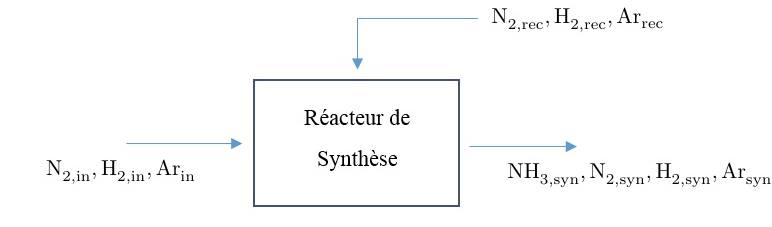
\includegraphics[scale=0.5]{media/reacteurNH3.jpg}
  \caption{Modélisation du recyclage des réactifs dans le réacteur de synthèse}
  \label{fig:purge}
\end{figure}

En développant le problème dans le cas d'un recyclage avec purge, on a :

\begin{align}
	\notag
	\begin{cases}
	 n_1 = \ce{N2_{,in} + N2_{,rec}} \\
	 n_2 = \ce{H2_{,in} + H2_{,rec}} \\
	 n_3 = \ce{Ar_{in} + Ar_{rec}} \\
	\end{cases}
	 &  \text{et}  &
	\begin{cases}
	 \ce{N2_{,syn}} = n_1 - \frac{x}{2} \\
	 \ce{H2_{,syn}} = n_2 - \frac{3x}{2} \\
	 \ce{NH3_{,syn}} = x \\
	 \ce{Ar_{syn} = Ar_{in} + Ar_{rec}} \\ 
	\end{cases}
	\\
\end{align}

Les équations de gauche sont dues au recyclage et celles de droite 
à la conservation de la matière. Ensuite, nous avons les trois relations
de la purge où nous posons un coefficient $k$ de proportion entre ce qui
est recyclé et ce qui sort du réacteur de synthèse. On fait l'hypothèse
que la purge enlève une proportion égale de moles pour chaque composé.

$$
\begin{cases}
 k\cdot \ce{N2_{,syn}} = \ce{N2_{,rec}} \\ 
 k\cdot \ce{H2_{,syn}} = \ce{H2_{,rec}} & k \in [0 \text{(ouvert)}, 1 \text{(fermé)}[ \\
 k\cdot \ce{Ar_{syn}} = \ce{Ar_{rec}} \\
\end{cases}
$$

Enfin, il nous reste à imposer que en régime l'argon rentrant doit être égal
à l'argon purgé. C'est indispensable pour éviter une accumulation du composé
dans le réacteur, et une baisse du rendement. 
Il faut donc : $(1 - k)\ce{Ar_{syn}} = \ce{Ar_{in}}$.

A partir de ces différentes équations, nous pouvons exprimer l'ammoniac
sortant en fonction des composants à l'entrée, du coefficient, de la pression
totale et de la température. Les détails du calcul sont laissés à l'attention 
du lecteur. Nous arrivons finalement à l'équation~\eqref{eq:finale}, qui peut
être résolue numériquement à l'aide de l'outil \textsc{Matlab}.  

\begin{align}
	K(T) & = \frac{4x\cdot p_0\cdot (\ce{N2_{,in} + H2_{,in} + Ar_{in}} - 
	\ce{NH3_{,syn}}(k + 1)) (1 - k)}{(\ce{2N2_{,in} - NH3_{,syn}})^{1/2} (\ce{2H2_{,in} - 3NH3_{,syn}})^{3/2} \cdot p_{tot}}
	\label{eq:finale}
\end{align}

Pour pouvoir complèter notre outil de gestion, nous exprimons les entrées 
en fonction du débit d'ammoniac voulue, de $k$, de la pression et de la
température. Pour cela nous nous plaçons dans le cas idéal stœchiométrique,
où aucuns des composants n'est en excès. De plus, nous prenons en compte la 
concentration d'argon naturellemnt dans l'air. 
 
$$
\begin{cases}
 \ce{N2_{,in}} = \ce{78Ar_{in}}\\ 
 \ce{N2_{,in}} = \ce{1/3H2_{,in}} \\
\end{cases}
$$

\section{Utilisation du logiciel \textsc{Aspen+}}
Nous avons ensuite utilisée le logiciel \textsc{Aspen+}
afin de simuler la synthèse de l'ammoniac. Pour cela
nous avons construit le flow-sheet présenté à la figure
\ref{fig:flow-sheet-aspen}. 

\begin{figure}
	\centering
	\rotatebox{90}{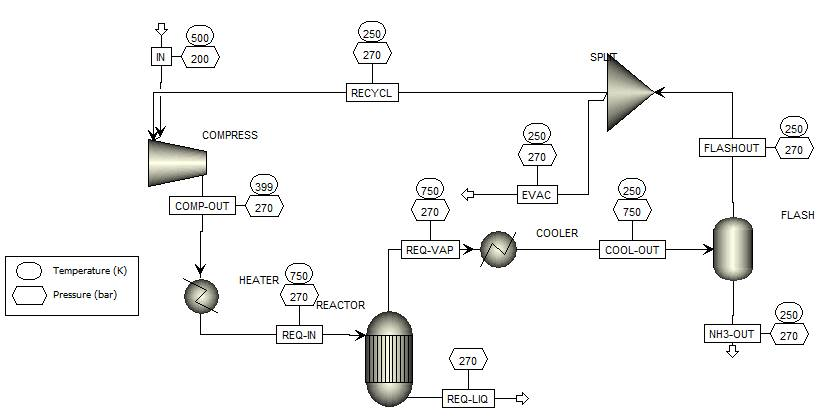
\includegraphics[scale=0.7]{media/flow-sheet.jpg}}
	\caption{Flow-sheet du procédé de synthèse de l'ammoniac
	réalisé avec \textsc{Aspen+}.}
	\label{fig:flow-sheet-aspen}
\end{figure}

% FIX : c'est bien cette méthode là?
Pour la simulation, nous avons utilisé la méthode
thermodynamique \textsc{SRK} qui est particulièrement
approprié pour les réactions entre gaz avec une pression
et une température élevée. Nous avons choisi d'utiliser
une purge de 4\%. La simulation nous fournit les résultats
présente à la figure \ref{fig:resultats-aspen}.

\begin{figure}
	\centering
	\rotatebox{90}{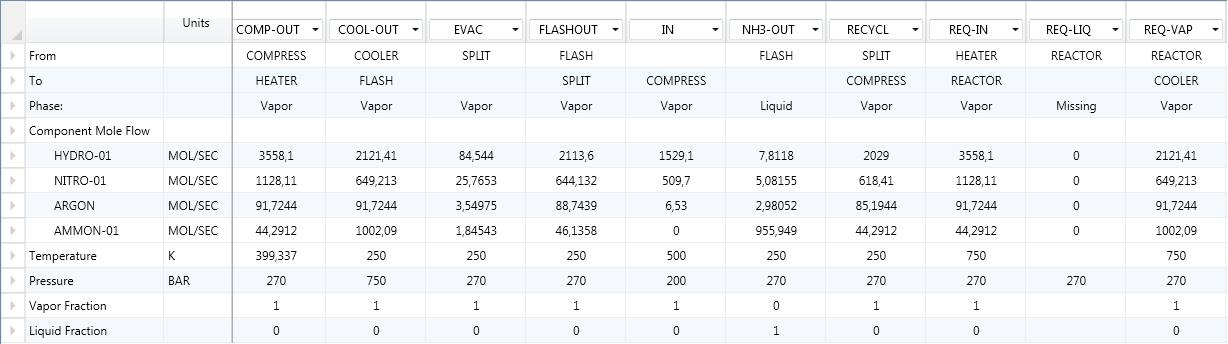
\includegraphics[scale=0.48]{media/results.jpg}}
	\caption{Résultats du procédé de synthèse de l'ammoniac
	réalisé avec \textsc{Aspen+}.}
	\label{fig:resultats-aspen}
\end{figure}

Ces résultats sont assez proches de ceux fournis par
l'outil de gestion. En effet, en prenant les valeurs
d'entrées nécessaires à la production à \unit{1000}{\kelvin} de
\unit{1500}{\ton\per\dday}, soit \unit{1019.40}{\mole\per\second},
de \chemform{NH_3} avec notre outil de gestion, notre simulation \textsc{Aspen+}
nous fournit un débit de \unit{955.949}{\mole\per\second} (ligne AMMON-01, colonne NH3-OUT),
soit un rendement de 93.77\%. Le débit de sortie de \chemform{NH_3}
est inférieur à celui obtenu avec notre outil de gestion étant donné que
ce dernier considère la réaction principale comme complète, tandis qu'\textsc{Aspen+}
rajoute la purge, nécessaire pour éviter l'accumulation d'\chemform{Ar}
mais ayant comme conséquence le défaussage d'une certaine quantité de
\chemform{N_2} et de \chemform{H_2}, et calcule également automatiquement un rendement
standard pour les réacteurs, séparateurs et tout composant de notre système
(nous pouvons d'ailleurs remarquer que la colonne NH3-OUT, indiquant le débit
de sortie supposé ne contenir que du \chemform{NH_3}, contient quand même du 
\chemform{N_2}, \chemform{H_2} et \chemform{Ar}, 
tout simplement parce qu'Aspen représente la réalité des choses et 
un séparateur n'est jamais parfait).
% TODO : >erreur<<<<< à calculer en % pour donner une meilleure idée => Quelle erreur? C'est plutôt un rendement non?
\end{document}

\chapter{Tache 3: Etude Hazop}
\documentclass{article}

% Langue
\usepackage[utf8]{inputenc}
\usepackage[T1]{fontenc}      
\usepackage[francais]{babel}

% Mise en forme générale
\usepackage[top=2.5cm,bottom=2.5cm,right=2.5cm,left=2.5cm]{geometry}

% Package divers
\usepackage{chemist} 
\usepackage[version=3]{mhchem}
\usepackage{chemfig}
\usepackage[squaren, Gray]{SIunits}
\usepackage{sistyle}
\usepackage[autolanguage]{numprint}
\usepackage{url}
\usepackage{rotating}
\usepackage{xcolor,colortbl}
\definecolor{Gray}{gray}{0.85}

\usepackage{hyperref}
\hypersetup{
    colorlinks,
    citecolor=black,
    filecolor=black,
    linkcolor=black,
    urlcolor=black
}

% Nouvelles commandes
\newcommand{\std}{\ensuremath{^{\circ}}}
\newcommand\ph{\ensuremath{\mathrm{pH}}}
\newcommand{\annexe}{\part{Annexes}\appendix}
\newcommand{\biblio}[1]{\bibliographystyle{plain}\bibliography{#1}\nocite{*}}

\newcommand{\doctitle}[1]{
	\title{#1}
	\author{\textbf{Groupe 124.3}\\
	\textsc{Frenyo} Péter (6266-12-00)\\
	\textsc{Gillain} Nathan (7879-12-00)\\
	\textsc{Lamine} Guillaume (7109-13-00)\\
	\textsc{Piraux} Pauline (2520-13-00)\\
	\textsc{Paris} Antoine (3158-13-00)\\
	\textsc{Quiriny} Simon (4235-13-00)\\
	\textsc{Schrurs} Sébastien (7978-13-00)}
	\date{\today}

	\begin{document}

	\maketitle
	\tableofcontents
}

\doctitle{Tache 4 : Etude HAZOP du noeud autour du réacteur de synthèse d'ammoniac}

\section{Dangers présentés par les substances mises en oeuvre durant la synthèse de l'ammoniac}
\subsection{L'azote}
Premièrement, le diazote utilisé est gardé sous pression. Tout gaz comprimé présente un danger. 
En effet, des rejets de gaz comprimé mal contrôlés dans les réacteurs chimiques peuvent entraîner 
la rupture des cuves, créer des fuites dans l'équipement ou les canalisations ou faire emballer la réaction \cite{canada}.
Si le contenant du gaz n'est de plus pas solidement fixé, cela peut entraîner un effet dit "fusée" 
et causer des dommages et blessures.

Le diazote est également un gaz toxique et peut entraîner des morts par asphyxie dans les espaces confinés. 
%il est nécessaire de vérifier la présence d'une proportion suffisante d'oxygène dans de tels espaces confinés 
%avant d'y pénétrer, ou de s'équiper d'un appareil respiratoire autonome. (Wikipedia) < Voit si tu veux rajouter ça en plus, ou c'est plutôt une solution.

\subsection{L'hydrogène}
Les dihydrogène étant également comprimé, il présente les même dangers de gaz sous 
pression que mentionnés pour le diazote.

De plus, le dihydrogène est un gaz extrêmement inflammable, réactif et explosif. 
Un choc, une étincelle ou autre peut facilement 
entraîner une combustion rapide pouvant menant à une explosion.

L'hydrogène peut également corroder certains métaux et être source de fragilités
ou fissures sur le matériel, et présente un danger de suffocation par inhalation.

\subsection{L'argon}
L'argon étant également maintenu sous pression, les même dangers que mentionnés
pour l'azote sont présents.

L'argon en forte concentration peut réduire la teneur en oxygène du milieu,
provoquant des pertes de consciences ou, dans le pire des cas, des morts par 
asphyxies \cite{canada}.

\subsection{L'ammoniac}
L'ammoniac est, encore une fois, maintenu sous pression, donc les dangers
des gaz sous pressions sont de nouveau présents ici.

L'ammoniac est également corrosif : son contact peut brûler et détruire 
les tissus, et peut également attaquer et corroder 
les métaux. Il est classé comme matière "très toxique ayant des effets 
immédiats graves". Il est irritant et toxique pour 
les êtres vivants et l'environnement \cite{canada}.

\section{Pourquoi n'y a-t-il pas de soupape de sécurité ou de disque de rupture sur
le réacteur de synthèses d'ammoniac?}
Dans le réaceur de synthèse, on a la réaction suivante : 

\begin{chemmath}
  3H_2(g) + N_2(g) \rightarrow 2NH_3(g)
\end{chemmath}

On peut donc voir que pour 4 moles de gaz de réactifs, 2 moles de gaz sont produites.
Puisque le nombre de moles de gaz diminue, la pression aura tendance à diminuer quand la réaction se fait. 
C'est pour cela qu'on ne craint pas la surpression et qu'aucun dispositif n'a été mis en place pour cela.

\section{Pourquoi y a-t-il des disques de rupture sur l'échangeur 124-MC ?}
En comparant les spécifications techniques des échangeurs de 
chaleur 124-MC\footnote{Pour localiser les différents composants cités dans cette section,
veuillez vous référer à la section \ref{sec:trajectoire}.} 
et 121-MC, on remarque que les pressions maximales
autorisées pour les coques extérieures ne sont pas identiques. 
En effet, la coque extérieure du second échangeur de chaleur (124-MC)
ne supporte pas une pression supérieure à approximativement \unit{17}{\kilo\pascal}
alors que l'autre échangeur peut supporter une pression jusqu'à 10 fois supérieure.
Or, même si les tubes supportent une pression identique à celle de la
coque de l'échangeur 124-MC, dans les deux cas, un mélange trop préssurisé
peut engendrer une rupture des tubes et de la coque de cette échangeur. 
C'est pourquoi, nous avons besoin d'un disque de rupture pour contrôler la presion.

\newpage
\section{Trajectoire du flux}
\label{sec:trajectoire}
La trajectoire des flux a été surlignée sur les trois figures
qui suivent. La figure \ref{pdf1} correspond au Process Flow Diagram
tandis que les deux autres figures, \ref{pid1} et \ref{pid2} 
correspondent aux Piping And Instrumentation Diagram.
Les trajectoires jaunes correspondent aux flux entrants sans ammoniac
tandis que les trajectoires bleues correspondent aux flux sortants
avec présence d'ammoniac.

\begin{figure}[htb!]
	\centering
	\rotatebox{90}{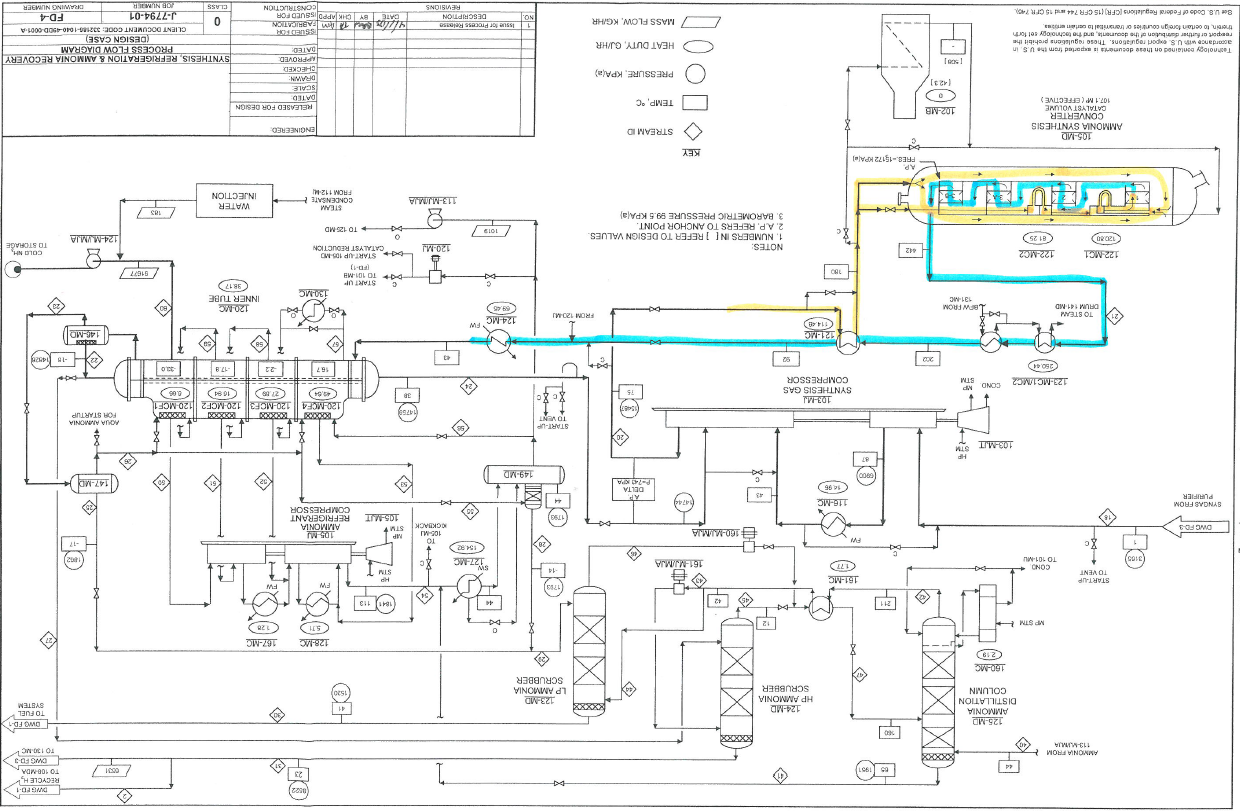
\includegraphics[scale=0.8]{media/pfd1.png}}
	\label{pdf1}
\end{figure}
\newpage

\begin{figure}[htb!]
	\centering
	\rotatebox{90}{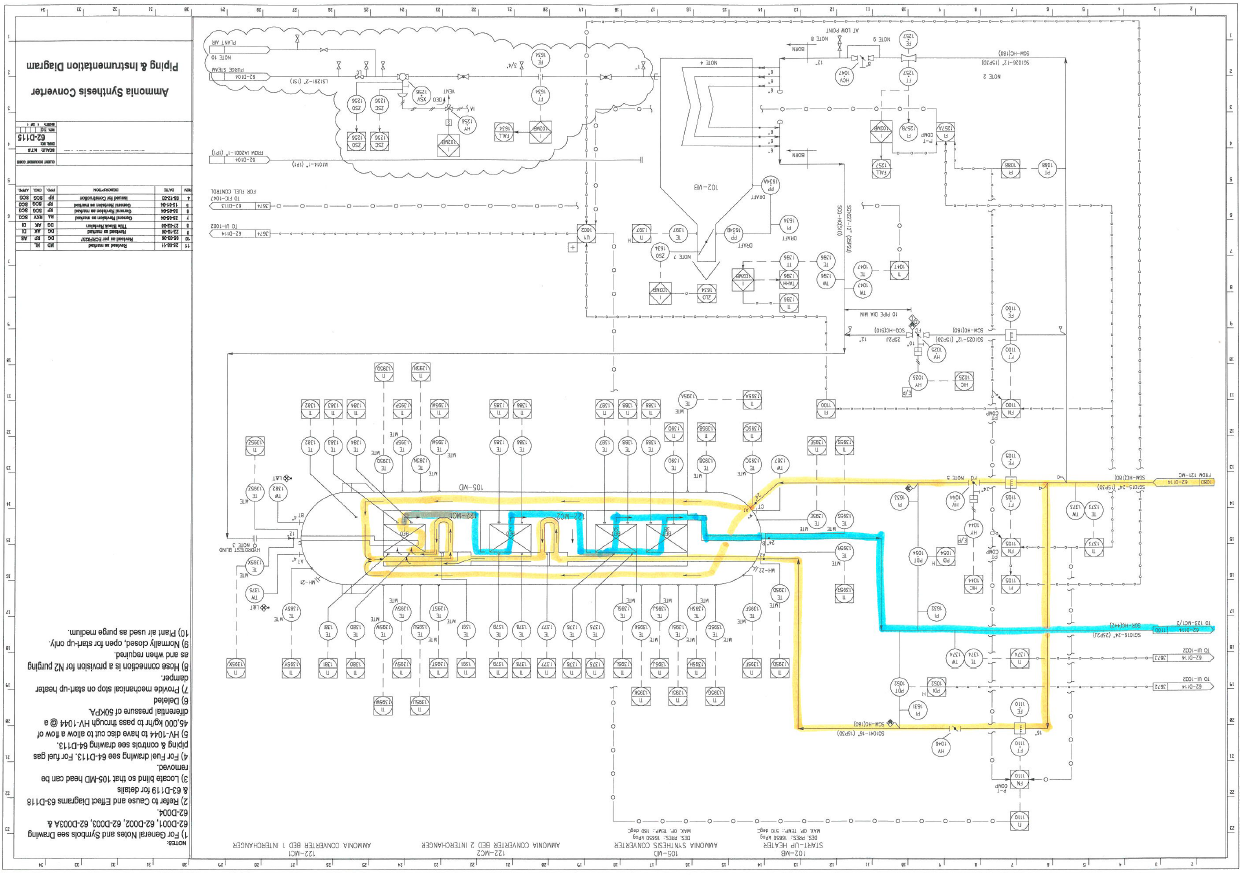
\includegraphics[scale=0.8]{media/pid1.png}}
	\label{pid1}
\end{figure}
\newpage

\begin{figure}[htb!]
	\centering
	\rotatebox{90}{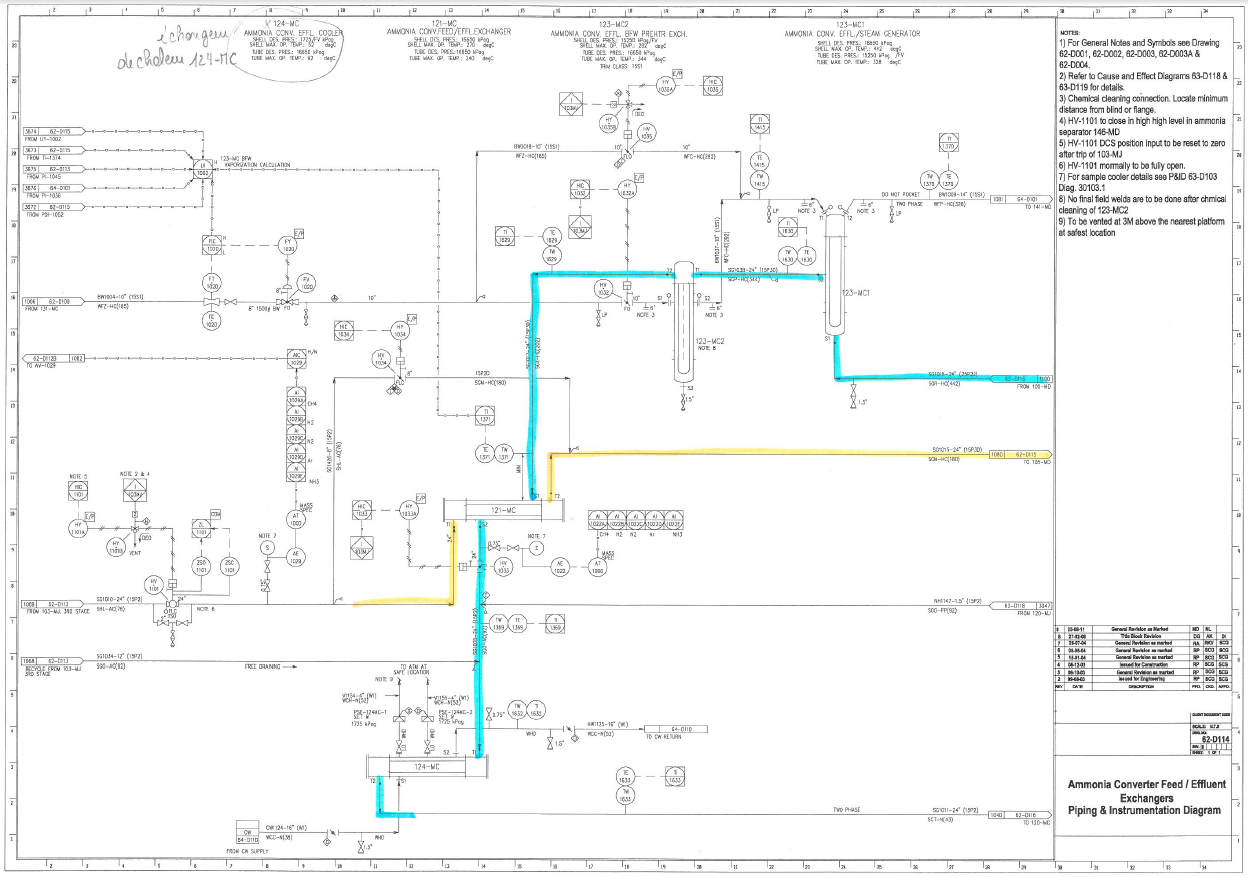
\includegraphics[scale=0.8]{media/pid2.png}}
	\label{pid2}
\end{figure}

\newpage
\section{Analyse HAZOP}
A nouveau, veuillez vous référer à la section \ref{sec:trajectoire}
pour localiser les différents composants cités dans cette section.

	\begin{table}[ht!]
		\centering
		\rotatebox{90}
		{
			\begin{tabular}{|p{0.25\textwidth}|p{0.25\textwidth}|p{0.25\textwidth}|p{0.25\textwidth}|}
				\rowcolor{Gray} Mot-guide		& Causes 	& Conséquences 	&	Mesures de maîtrise 	\\
				\hline
				Trop de corrosion		 
				& Une \textit{hydrogen attack} due à réaction à haute pression 
				de l'hydrogène avec l'acier. Lieu: Du début jusqu'à la chambre 1 du 105MD
				& Les tuyaux sont endommagés (percés ou présence du fuites) ce qui peut
				même mener à une explosion quand l'hydrogène et l'oxygène rentrent en contact. 
				Lieu : Du début jusqu'à la chambre 1 du 105MD.	 
				& Contrôle des matériaux	et augmentation de leur qualité. Prévoir les revêtements adéquats pour éviter tout contact entre acier et hydrogène. 	\\				
				\hline
				Température	trop basse	
				& Liquéfaction/condensation de l'ammoniac juste après le 124MC.	
				& Tuyaux bouchés ce qui peut entrainer une surpression juste après le 124MC.  
				& Installer un dispositif (disque de rupture ou soupape de sécurité) pour contrer
					les problèmes de surpression. \\
				\hline 
				Trop d'usure, corrosion	
				& Dégradation des installations avec le temps et impureté des produits 
				dans les conduits. Lieu: Dans toutes les canalisations mais principalement entre 
				le 105MD et le 123MC1 du à la haute pression.	
				& Entraîne des réactions indésirées qui amènent des impuretés dans l'ammoniac. 
				Lieu : Dans toutes les canalisations mais principalement entre le 105MD et le 123MC1 
				du à la haute pression.	 
				&  Contrôler les installations tous les ans et mettre un filtre physique pour avoir de l'ammoniac pur.	\\
				\hline
				Température trop haute	
				&	Surpression dans le réacteur de synthèse d'ammoniac (105MD).				
				& Peut entrainer des fissures dans la paroie voir même la destruction du réacteur. 
				Il y alors risque d'explosion (105MD).							
				& Présence d'un disque de rupture pour éviter la surpression. \\
				\hline
			\end{tabular}
		}
		\caption{Synthèse de l'analyse HAZOP.}
	\end{table}

\newpage
\biblio{sources-tache4}

\end{document}
\chapter{Tache 5: dimensionnement d'une soupape de sécurité}
\documentclass{article}

% Langue
\usepackage[utf8]{inputenc}
\usepackage[T1]{fontenc}      
\usepackage[francais]{babel}

% Mise en forme générale
\usepackage[top=2.5cm,bottom=2.5cm,right=2.5cm,left=2.5cm]{geometry}

% Package divers
\usepackage{chemist} 
\usepackage[version=3]{mhchem}
\usepackage{chemfig}
\usepackage[squaren, Gray]{SIunits}
\usepackage{sistyle}
\usepackage[autolanguage]{numprint}
\usepackage{url}
\usepackage{rotating}
\usepackage{xcolor,colortbl}
\definecolor{Gray}{gray}{0.85}

\usepackage{hyperref}
\hypersetup{
    colorlinks,
    citecolor=black,
    filecolor=black,
    linkcolor=black,
    urlcolor=black
}

% Nouvelles commandes
\newcommand{\std}{\ensuremath{^{\circ}}}
\newcommand\ph{\ensuremath{\mathrm{pH}}}
\newcommand{\annexe}{\part{Annexes}\appendix}
\newcommand{\biblio}[1]{\bibliographystyle{plain}\bibliography{#1}\nocite{*}}

\newcommand{\doctitle}[1]{
	\title{#1}
	\author{\textbf{Groupe 124.3}\\
	\textsc{Frenyo} Péter (6266-12-00)\\
	\textsc{Gillain} Nathan (7879-12-00)\\
	\textsc{Lamine} Guillaume (7109-13-00)\\
	\textsc{Piraux} Pauline (2520-13-00)\\
	\textsc{Paris} Antoine (3158-13-00)\\
	\textsc{Quiriny} Simon (4235-13-00)\\
	\textsc{Schrurs} Sébastien (7978-13-00)}
	\date{\today}

	\begin{document}

	\maketitle
	\tableofcontents
}

\usepackage[numbered, framed]{mcode}
\doctitle{Tache 5 - Dimensionnement d'une soupape de
sécurité pour un tank de stockage d'ammoniac}

\section{Enoncé}
Un stockage d’ammoniac (\ce{NH3}) liquide est
situé à proximité du stockage de mazout du site.
Suite à une fuite sur ce dernier et de l’ignition
de celle-ci, un feu de flaque pourrait se développer
autour du tank d’ammoniac.  Vous avez pour mission
de dimensionner une soupape de sécurité à installer
sur le tank d’ammoniac de manière à protéger celui-ci
contre les effets d’une surpression consécutive à 
l’effet du feu sur le tank.

\subsection{Données}
Nous disposons des données numériques suivantes :

\begin{itemize}
	\item Le tank est de forme cylindrique vertical à 
	extrémités hémisphériques et est situé au sol ;
	\item Hauteur total du tank : \unit{12}{\meter} ;
	\item Niveau de \ce{NH_3} dans le tank : \unit{8}{\meter} ;
	\item Diamètre du tank : \unit{6}{\meter} ;
	\item Température normale de stockage : \unit{20}{\degreecelsius} ;
	\item Rapport des capacités calorifiques à pression
	et à volume constante ($\frac{C_p}{C_v}$) du \ce{NH_3} : 1.33 ;
	\item Pression de design\footnote{Pression maximale
	que le tank peut supporter.} : \unit{15}{\bbar g}\footnote{L'unité
	\unit{}{\bbar g} est une unité de pression relative, mesurée par 
	rapport à la pression atmosphérique (à savoir \unit{1}{\bbar}). Pour
	retrouver la pression absolue, il suffit donc d'ajouter \unit{1}{\bbar}
	à la pression relative.} ;
	\item Facteur de compressibilité $Z = 1.0$ ;
	\item La soupape sera une soupape conventionnelle et 
	la contrepression sera nulle ;
	\item Lu'sine est munie de système de drainages des fuites 
	et d'un équipement moderne de lutte contre l'incendie.
\end{itemize}

Nous disposons également des deux graphes suivants :

\begin{figure}[htb!]
	\centering
	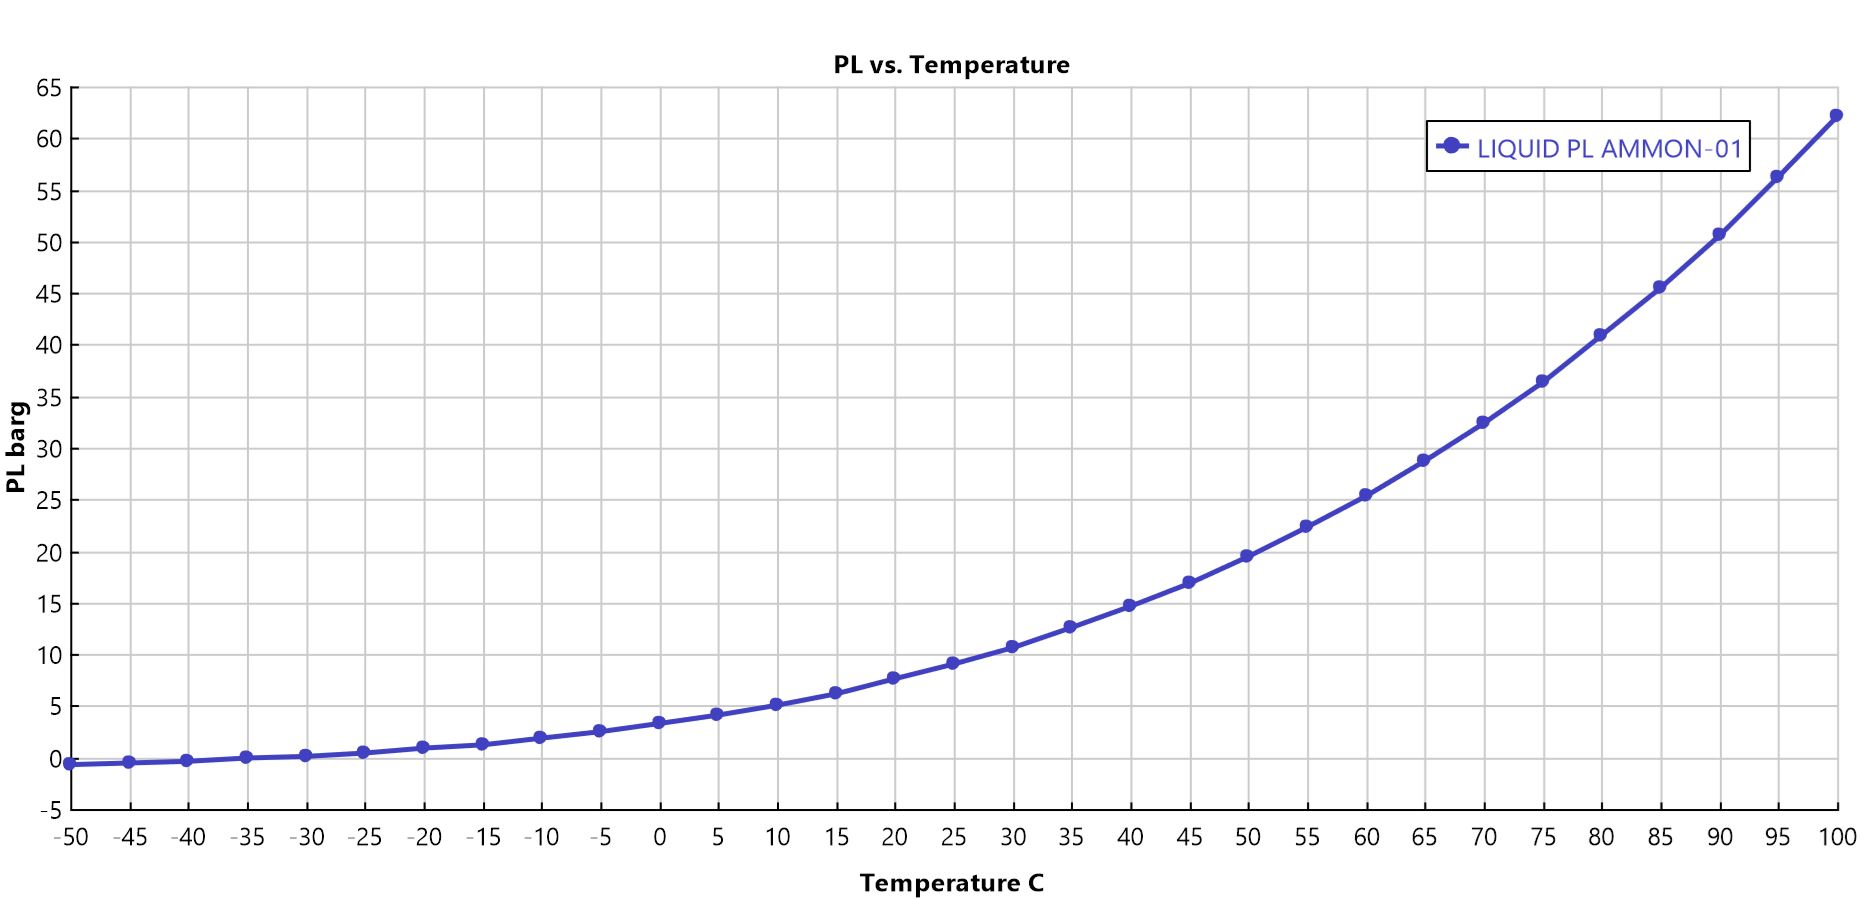
\includegraphics[scale=0.45]{media/PL_vs_temperature.jpg}
	\caption{Graphe de la tension de vapeur (en \unit{}{\bbar g})
	par rapport à la température (en \unit{}{\degreecelsius}).}
	\label{pvst}
\end{figure}

\begin{figure}[htb!]
	\centering
	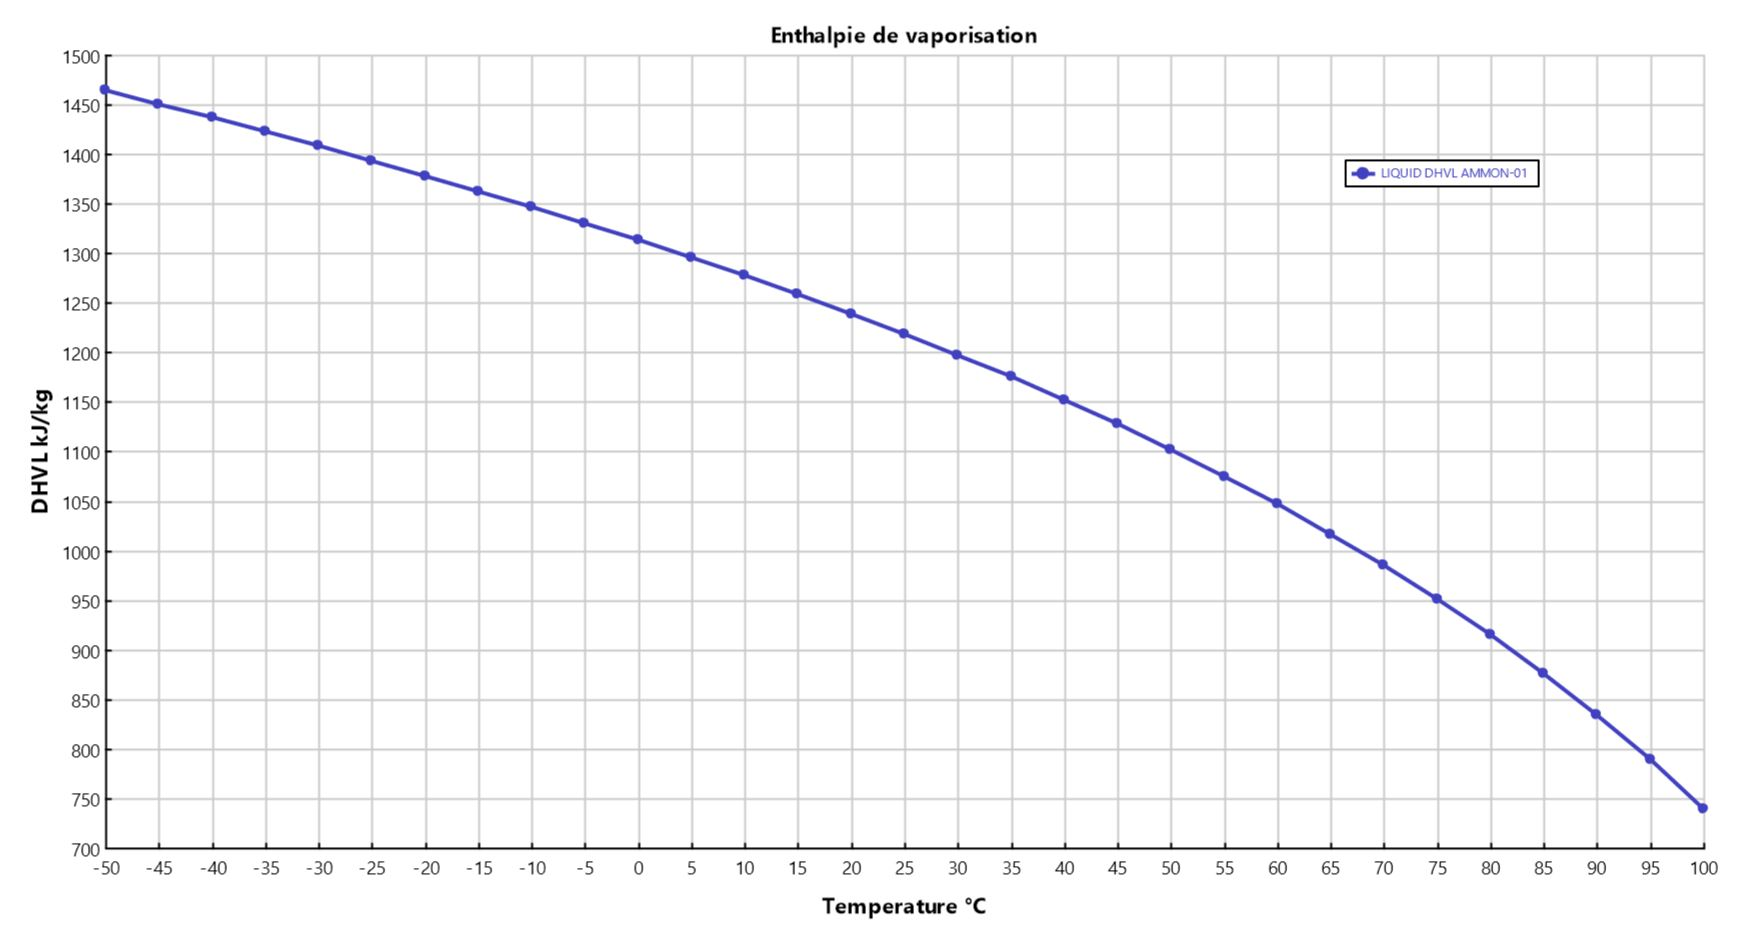
\includegraphics[scale=0.49]{media/enthalpie_vap.jpg}
	\caption{Graphe de l'enthalpie de vaporisation 
	(en \unit{}{\kilo\joule\per\kilo\gram}) par rapport à
	la température (en \unit{}{\degreecelsius}).}
	\label{vap}
\end{figure}

\section{Questions}
\paragraph{Quelle est la pression normale de stockage?}
La température normale de stockage étant de \unit{20}{\degreecelsius}
et la pression à l'intérieur du tank étant égale à la tension
de vapeur de l'ammoniac, on trouve, via la figure
\ref{pvst} 

$$p_{\text{normale}} \approx \unit{8}{\bbar g} = \unit{9}{\bbar}.$$

\paragraph{Quelle sera la pression de stockage en été 
(\unit{30}{\degreecelsius})?}
A nouveau, en s'aidant de la figure \ref{pvst}, on trouve

$$p_{\text{été}} \approx \unit{11}{\bbar g} = \unit{12}{\bbar}.$$

\paragraph{Quelle sera la pression maximale de tarage
de la soupape de sécurité?}
La pression maximale de tarage est égale à la pression de 
design du tank, c'est à dire

$$p_{\text{tarage, max}} = \unit{15}{\bbar g} = \unit{16}{\bbar}.$$

Pour les trois questions suivantes, on considère la pression
de tarage de la soupape comme étant égale à \unit{16}{\bbar}.

\paragraph{Quelle sera la pression durant la décharge?}
Dans le cas d'un incendie, la surpression autorisée est de 121\%
de la pression de tarage \cite{mignon}, à savoir 

$$p_{\text{décharge}} = \unit{19.36}{\bbar}$$

dans notre cas.

\paragraph{Quelle sera la température du liquide durant
la décharge via la soupape?}
A partir de le figure \ref{pvst}, on trouve 

$$T \approx \unit{49.5}{\degreecelsius} = \unit{322.65}{\kelvin}.$$

\paragraph{Quelle sera la taille de la soupape nécessaire?}
La taille de l'orifice de la soupape se calcule en utilisant la formule
suivante\cite{mignon} 

$$A = \frac{W}{CK_dP_1K_bK_c}\sqrt{\frac{TZ}{M}}.$$

Afin d'y voir plus clair, listons dans un premier temps 
tous les paramètres connus et convertissons, si nécessaire,
leurs unités selon les besoins de la formule.

\begin{itemize}
	\item $K_d$ est le coéfficient de décharge. Pour un gaz,
	on a $K_d = 0.975$ ;
	\item $P_1$ est la préssion durant la décharge, on a donc
	$P_1 = p_{\text{décharge}} = \unit{19.36}{\bbar} = 
	\unit{19.36\cdot10^2}{\kilo\pascal}$ ;
	\item $K_b$ est un facteur de correction dû à contrepression. 
	Sa valeur pour une soupape conventionnelle comme la nôtre est de 1 ;
	\item $K_c$ est un facteur de correction dû aux éventuelles
	combinaisons soupape/disque de rupture. Dans notre cas, $K_c = 1$ ;
	\item $T$ est la témpérature de décharge, c'est à dire 
	\unit{322.65}{\kelvin} ;
	\item $Z = 1$ ;
	\item $M$ est la masse moléculaire, on calculer assez 
	simplement que $M = \unit{17}{\kilo\gram\per\kilo\mole}$.
\end{itemize}

% FIXME : c'est quoi C ?
Occupons-nous maintenant des paramètres inconnus : $C$ et $W$,
qui est débit massique relâché.
La premier peut être calculé à partir de la formule suivante\cite{mignon}

$$C = 0.03948\sqrt{k\frac{2}{k+1}^{\frac{k+1}{k-1}}}$$

où $k = \frac{C_p}{C_v} = 1.33$. On a donc $C = 0.02655536953$.

Le deuxième est un petit peu plus compliqué à obtenir. Pour obtenir
$W$, nous allons utiliser la formule suivante\cite{mignon}

$$W = \frac{Q}{\Delta H_{\text{vap}}(T_{\text{décharge}})}$$ 

où $\Delta H_{\text{vap}}(T_{\text{décharge}}) \approx 
\unit{1115\cdot10^3}{\joule\per\kilo\gram}$ est trouvé en utilisant
la figure \ref{vap}. Pour calculer $Q$, qui correspond à
l'absorption totale de chaleur par les surfaces en contact avec
l'ammoniac liquide (exprimé en \unit{}{\watt}) nous pouvons
utiliser la formule suivante\cite{mignon}

$$Q = C_1FA_{\text{ws}}^{0.82}$$

où $C_1 = 43200$ est une constante, $F$ est un 
facteur d'environnement et $A_{\text{ws}}$ correspond
à l'aire de la \textit{wetted surface}, autrement dit
il s'agit de la surface totale en contact avec l'ammoniac
liquide. On peut trouver la valeur de $F$ dans des tables
\cite{mignon}. Dans notre cas, le tank n'étant pas isolé,
on trouve $F = 1.0$.

Calculons maintenant $A_{\text{ws}}$. Avant tout, il faut
savoir qu'on considère qu'il n'y a plus d'absorption de chaleur
à \unit{7.62}{\meter} au dessus du feu\cite{mignon}.
$A_{\text{ws}}$ est constitué de deux surfaces ; la partie
basse du tank constitué de l'hémisphère et la partie centrale
constitué du cylindre. L'hémisphère de rayon égale à \unit{3}{\meter}
a une surface de \unit{56.54866776}{\meter\squared} et la partie
cylindrique d'une hauteur de \unit{4.62}{\meter} a une surface
de \unit{87.08494836}{\meter\squared}. On a donc finalement 
$A_{\text{ws}} = \unit{143.6336161}{\meter\squared}$.

On trouve dès lors que $Q = \unit{2537661.812}{\watt}$.
On fini enfin par obtenir 

$$W = \unit{2.275929876}{\kilo\gram\per\second} =
\unit{8193.347554}{\kilo\gram\per\hour}.$$

Nous disposons maintenant de toutes les informations nécessaires
pour calculer $A$ :

$$A = \unit{712.0990948}{\milli\meter\squared}.$$

\paragraph{Si la pression de design de l'équipement était de \unit{20}{\bbar g},
quel serait l'effet d'augmenter la pression de tarage de \unit{5}{\bbar} et de 
la porter à \unit{20}{\bbar g}?}
Afin d'éviter de refaire tous les calculs (et les divers changement d'unités)
pouvant aboutir à un grand nombre d'erreurs de calculs et de conversion, nous
avons créer une fonction Matlab permettant de calculer la taille de l'orifice
automatiquement (présente en annexe \ref{code-matlab}. Cette fonction prend 4 paramètres en argument : la pression
de tarage en bars absolu, la température de décharge en Kelvin (mesurable sur
la figure \ref{pvst}), l'enthalpie de vaporisation correspondant
à la température de décharge en kilojoules (mesurable sur la figure \ref{vap}) et un dernier
paramètre dont la valeur vaut 1 pour cette question\footnote{Ce paramètre $F$ dépend
de l'isolement thermique du réservoir, ici on suppose qu'il n'est pas isolé.}.
Dans ca cas ci, la pression de tarage vaut \unit{21}{\bbar}. La pression
de décharge valant, dans le cas d'un incendie, 121\% de ma pression de tarage,
on peut trouver la température de décharge et l'enthalpie de vaporisation
correspondante. On trouve $T_{\text{décharge}} = \unit{58}{\degreecelsius}$
et $\Delta H_{\text{vap}}(T_{\text{décharge}}) = \unit{1050}{\kilo\joule\per\kilo\gram}$.
En rentrant ces 3 paramètres dans notre fonction, on trouve 

$$A = \unit{578.06}{\milli\meter\squared}.$$

\paragraph{Pour la première pression de tarage, quelle est l'influence
d'isoler thermiquement le tank avec un isolant tel que le coefficient
d'échange avec l'extérieur soir réduit à une valeur de
\unit{10}{\watt\per\meter\squared\kelvin}?}
Le coefficient d'échange avec l'extérieur correspond à

$$\frac{Q}{A_{\text{WS}T}} = \frac{C_1FA_{\text{WS}}^{0.82}}{A_{\text{WS}}T}.$$

En égalant ce coéfficient à 10, on trouve $F = 0.1826$.
On rentrant ces valeurs dans notre fonction, on trouve 

$$A = \unit{130}{\milli\meter\squared}$$

soit plus de 5 fois moins que sans isolation thermique.

\biblio{sources-tache5}
\appendix
\section{Code Matlab utilisé}
\label{code-matlab}
\lstinputlisting{matlab/SizePSV.m}
\end{document}
\chapter{Tache 7: Rapport des activités de terrain}
\documentclass{article}

% Langue
\usepackage[utf8]{inputenc}
\usepackage[T1]{fontenc}      
\usepackage[francais]{babel}

% Mise en forme générale
\usepackage[top=2.5cm,bottom=2.5cm,right=2.5cm,left=2.5cm]{geometry}

% Package divers
\usepackage{chemist} 
\usepackage[version=3]{mhchem}
\usepackage{chemfig}
\usepackage[squaren, Gray]{SIunits}
\usepackage{sistyle}
\usepackage[autolanguage]{numprint}
\usepackage{url}
\usepackage{rotating}
\usepackage{xcolor,colortbl}
\definecolor{Gray}{gray}{0.85}

\usepackage{hyperref}
\hypersetup{
    colorlinks,
    citecolor=black,
    filecolor=black,
    linkcolor=black,
    urlcolor=black
}

% Nouvelles commandes
\newcommand{\std}{\ensuremath{^{\circ}}}
\newcommand\ph{\ensuremath{\mathrm{pH}}}
\newcommand{\annexe}{\part{Annexes}\appendix}
\newcommand{\biblio}[1]{\bibliographystyle{plain}\bibliography{#1}\nocite{*}}

\newcommand{\doctitle}[1]{
	\title{#1}
	\author{\textbf{Groupe 124.3}\\
	\textsc{Frenyo} Péter (6266-12-00)\\
	\textsc{Gillain} Nathan (7879-12-00)\\
	\textsc{Lamine} Guillaume (7109-13-00)\\
	\textsc{Piraux} Pauline (2520-13-00)\\
	\textsc{Paris} Antoine (3158-13-00)\\
	\textsc{Quiriny} Simon (4235-13-00)\\
	\textsc{Schrurs} Sébastien (7978-13-00)}
	\date{\today}

	\begin{document}

	\maketitle
	\tableofcontents
}

\doctitle{Projet 3 - Tache 2}

\section{Introduction}
Dans le cadre du projet, vous avons eu l'opportunité de
participer à diverses activités en lien avec la chimie ou
le travail en équipe. Ce document présente les rapports,
destinés aux membres du groupes, de ces différentes visites.

\section{Visite du plant de Yara à Tertre}

\subsection{Introduction}
L’usine de Tertre fait partie de l’entreprise \textsc{Yara}. L’entreprise norvégiene est l’un des plus grands producteurs
mondiaux d’engrais azotés. Le site de Terte date de fin des années 60. L’usine a fait le choix de produire sur place 
l’ammoniac qui lui est nécessaire à la production d’engrais, 99 \%  de sa production est utilisé sur le site de l’usine. 
La production d’ammoniac dépendant de l’apport en méthane, l’usine s’est établie à Tertre pour sa bonne localisation 
géographique par rapport aux principaux transports de gaz en Belgique. L'usine qui fait partie des plants éfficaces malgré 
sa vétustée, permet de produire \unit{1150}{\ton\per\dday} d’amoniac en utilisant le désign de Kellogg. 
Toutefois, un plant moderne peut produire jusqu’à \unit{3000}{\ton\per\dday} de NH3.

\subsection{Réactifs et produits}

\subsubsection{Azote}

Pour obtenir de l’azote, l’usine fixe celui contenu dans l’air ($\unit{946}{\kilo\joule} + N_2 \longrightarrow 2N$). 
Il y a en moyenne 76 à 78\% d’azote dans l’air extérieur. C’est un gaz asphyxiant inodore, incolore et volatile. 

\subsubsection{Hydrogène}
Il est stocké sous haute pression : 200 bars et à une température de \unit{500-600} {\degreeCelsius}.
L’hydrogène est un produit très dangereux. Il peut se révéler explosif au contact de l’oxygène. Dans l’état de haute 
pression dans lequel il se trouve il peut donner lieu à une réaction: 

\begin{chemmath} 
\ Fe_3C(=acier) + 2H_{2} \longrightarrow CH_4 + 3Fe
\end{chemmath} 

\begin{chemmath} 
\ N_2(g) + 3H_{2}O(g) \longrightarrow 2NH_3(g)
\end{chemmath} 

C’est ce qui s’appelle une « hydrogen attack ». A haute pression, il va décomposer l’acier ce qui entraine une 
fragilisation des tuyaux et peut amener à une explosion. Une conséquence indispensable à la sécurité est qu’il faut choisir 
les bons matériaux de tuyauterie.

\subsubsection{Ammoniac}

Ce composé incolore est plus léger que l’air et est assez facile à liquéfier.  Sa température critique 
(température à laquelle on ne peut dissocier le composé sous sa forme liquide et gazeuse) est de \unit{132.4}{\degreeCelsius},
sa pression critique est de 113 bars . Point de vue sécurité, le contact chimique avec les muqueuses peut se révéler 
dangereux. On parle de 5ppm d’exposition  pour permettre une durée d’exposition illimitée.

\subsection{Réaction}

\subsubsection{Reformage primaire}

Une désulfurisation est d’abord effectuée pour éviter toute une série de problème dans la suite du processus, par exemple
l’empoisonnement des catalyseurs. Lors du reformage primaire, le méthane est « craqué » en dihydrogène. A la fin de cette
étape il ne reste plus que 12 \% de méthane qui n’a pas été dissocié. Il est indispensable d’avoir un excès de vapeur sinon 
on aura une formation de coke c’est-à-dire du carbone pur ou charbon. Cela entraine un encrassement de toute l’installation 
et un arrêt du processus obligatoire.
Le catalyseur utilisé pour cette réaction est le nickel. Pour la sécurité, il y a présence d’un « safety manager » qui est 
une installation automatique reliée à des détecteurs de fuites. De plus, l’installation est arrêtée tous les quatre ans pour
maintenance. A part ça, l’usine marche 24h/24 7j/7. Après un arrêt, il faut 3-4 jours pour lancer le processus.

\subsubsection{Reformage secondaire}

Le procédé est identique à celui que nous effectuons dans notre projet. Le méthane qui n’avait pas réagi est presque
entièrement dissocié. Etant donné que la température est beaucoup plus haute, il faut une protection réfractaire et une
« chemise d’eau » pour éviter les chocs thermiques. A part cela, le réacteur a douze ans de vie.
A la suite du reformage, ils réutilisent la chaleur des gaz qui sortent pour chauffer toutes sortes de sous-installations
dans le but d’avoir le moins de perte d’énergie possible. Les deux étapes qui vont suivre consistent à purifier les deux 
réactifs que l’on a déjà obtenus. 

\subsubsection{HTS \& LTS: décompression}

Le monoxyde de Carbonne est transformé en dioxyde de Carbonne car ce dernier est plus facile à éliminer. On va baisser 
la pression pour « flasher » le dioxyde de Carbonne de la même manière qu’on secoue une bouteille de coca pour en extraire
le gaz. Ensuite on élimine le dioxyde de Carbonne obtenu en le rejetant tout simplement dans l’air ce qui est évidemment
très polluant. 

\subsubsection{Méthanateur}

On purifie le flux de gaz en faisant la réaction inverse. Cela va produire du méthane qu’on va récolter et renvoyer 
au début du cycle.  On élimine également les derniers composés oxygénés résiduels qui sont dangereux pour la synthèse 
proprement dite de l’ammoniac.

\subsubsection{Synthèse}

%je dois encore mettre une figure ici

Le gaz est à 128 bars à l’entrée du réacteur. Après notre tri il n’y a théoriquement plus que de l’azote, de 
l’hydrogène, de l’ammoniac à l’équilibre ainsi que les gaz inertes (Argon principalement). Lors de la réaction, après une
première augmentation de la température on refroidit le mélange pour ensuite le réchauffer. En fait, La réaction se fait en 
plusieurs plateaux successifs pour augmenter le rendement en ammoniac. La réaction est également favorisée par des catalyseurs 
au fer. Grace à leurs micropores, ils possèdent de grandes surfaces de contact pour que les molécules réagissent entre elles.
L’énergie d’activation diminue sans changer le chemin réactionnel. Ils supportent et favorisent la rencontre des molécules 
en créant des sites de rencontres.
Malgré toute ces opérations on obtient que 14\% d’ammoniac c’est pourquoi on recycle les composants qui n’ont pas réagis.  
Les composants étant réintroduis dans le réacteur, la pression va augmenter et les résidus de gaz comme l’argon et l’hélium 
vont augmenter. Il y a à Tertre 12 à 14\% de gaz inertes à purger grâce à une vanne. Il faut procéder à une purge automatique. 
On peut enfin stocker l'ammoniac par procédé cryogénique ou bien sous haute pression.


\subsection{Aspect écologique}

L’usine  est assez polluante. Elle rejette beaucoup de monoxyde de Carbonne, la solution de Lumine utilisée pour
l’absorption du monoxyde de Carbonne n’est pas très écologique ainsi que les hydrocarbures que les machines utilisent.
L’usine n’est également pas tout à fait optimisée, il y a notamment des pertes au niveau des bruleurs.


\section{Visite du centre Total Research Technology Feluy}
Chaque année, \textsc{Total} investit plus de 8 milliards de
dollars dans des centres de recherches comme celui de Feluy.
Dans ce centre, les recherches effectuées portent sur les
conditions d'opérations et les catalyseurs utilisés lors de
la fabrication de polymères. Lorsque les ingénieurs de chez
Total veulent tester de nouvelles conditions d'opérations
(température, pression, etc) ou tester un nouveau catalyseur,
ils le font d'abord sur des petites unités, qu'on appelle unités
pilotes. Ces unités permettent de produire une petite quantité
de polymère (de l'ordre de quelques centaines de grammes). Si
ces premiers tests sont concluants, ils passent ensuite sur une
plus grosse unité pilote capable de produire \unit{50}{\kilo\gram
\per\dday}. La taille d'une telle unité pilote est vraiment
impressionnante. On pourrait s'attendre à un petit réacteur situé
dans un laboratoire, mais en réalité l'unité pilote mesure une dizaine
de mètre de hauteur et s'étale sur au moins \unit{40}{\meter\squared}.
On imagine à peine la taille de l'unité de production qui produit
des tonnes de polymères par jour.

Cette visite, bien que très intéressante et très instructive, n'était
malheureusement pas en lien avec notre projet.

\section{Visite de la station de biométhanisation de l'AIVE à Tennevile}
\subsection{Introduction}
Le centre de gestion des déchets de Tenneville a pour but de valoriser les 
déchets verts et organiques qu’il recueille des ménages wallons des provinces de 
Liège, Namur et Luxembourg. La population concernée est alors conviée à trier ses déchets 
au préalable afin d’optimiser le processus de valorisation au maximum. 
Ainsi, ce sont environs 240.000 tonnes de déchets (verts et PMC) qui sont récoltés 
au centre chaque année, dont 30 000 tonnes de déchets ménagers. De l’énergie est alors produite, 
d’abord sous forme de biogaz, et ensuite sous forme de chaleur et d’électricité exploitables 
dans d’autres applications du site.

\subsection{Production de biogaz}
Toute la masse de déchets ménagers est alors d’abord entreposée dans de grands hangars, 
pour assurer une première phase de décomposition. On estime alors la proportion de plastique 
à environ 0.1 – 0.5\% de la masse totale. Afin d’accélérer le processus sans devoir retourner 
les tas de déchets mécaniquement, on souffle de l’air par en-dessous dans le but qu’un maximum 
de matière soit en contact constant avec de l’air. Après 2-3 semaines d’entreposage sur 
les « dalles », le digestat est filtré par un procédé de tamisage destiné à se séparer d’un maximum de déchets plastiques. 

Par la suite, ces déchets sont alors traités de sorte à produire environs 3.6 millions de m^3 
de biogaz par an, composé à 55\% de méthane. Moyennant un certain investissement, il 
serait possible d’augmenter la teneur en méthane du biogaz, et d’ainsi le rendre utilisable 
pour une plus grande série d’applications.
Or en réalité, le gaz produit ici étant ici destiné à faire fonctionner des moteurs à gaz prévus à cet effet, 
une meilleure qualité n’est donc pas nécessaire. Dans le cas du centre à Tenneville, les moteurs 
à gaz sont destinés à produire de l’électricité (7000MW/an) et de la chaleur à partir de biogaz 
contenant cette proportion-là de méthane. Aucun besoin d’en améliorer la qualité. 

Cependant, à sa sortie, le biogaz est très chargé en humidité (environ 100\% d’humidité relative) 
ce qui n’est pas enviable compte tenu des moteurs utilisés. Afin d’enlever une bonne partie d’eau contenue 
dans le gaz, on le refroidit brusquement. L’eau va ainsi condenser, et il suffira alors de récupérer 
le gaz, alors moins humide. Le gaz ainsi produit est ensuite utilisé pour produire de l’énergie, 
qui est alors réinjectée dans le reste du centre pour par exemple chauffer les bureaux, 
fournir les ordinateurs en électricité ou encore alimenter diverses autres productions présentes 
sur le sites (séchage des boues, production de compost, etc).

\subsection{Conclusion}
Cette visite nous aura au moins permis de prendre connaissance d’une façon plutôt économique de 
produire du méthane. En effet, moyennant un traitement décrit plus haut, il est possible d’obtenir
du biogaz à partir de déchets organiques ménagers. Nul besoin donc d’investir dans des matières 
premières coûteuses, d’autant qu’une certaine aide de la part des autorités est envisageable, 
compte tenu du fait que ce sont des déchets publics qui sont pris en charge.



\section{Laboratoire d'électrolyse}
\subsection{Découverte d'un autre procédé de fabrication du dihydrogène : l'électrolyse}
Le but du laboratoire était de découvrir un nouveau procédé de
fabrication du dihydrogène autre que le vaporéformage, de le
caractériser et de le comparer avec le procédé utilisé dans la
méthode de production Haber-Bosch en terme de consommation, de
pollution et de coût de production.

\subsection{Explication de la réaction}
L'électrolyse de l'eau consiste à briser les liaisons entre
l'oxygène et l'hydrogène de l'eau à l'aide d'un courant électrique.
Ensuite, les deux composés prennent part à une réaction d'oxydo-réduction.
Ce qui donne, à température ambiante, de l'hydrogène sous forme de
dihydrogène gazeux (tout comme l'oxygène qui devient du dioxygène gazeux),
un des produits souhaités. Le réaction suivante est la réaction bilan du
procédé en question.

\begin{chemmath}
	2H_2O(l) \rightleftharpoons 2 H_2(g) + O_2(g)
\end{chemmath}

En décomposant la réaction selon ce qui passe à l'anode et à la cathode,
on obtient :

\begin{chemmath}
	2H^+(aq) + 2 e^- \rightleftharpoons H_2(g)
\end{chemmath}

à la cathode et

\begin{chemmath}
	2H_2O(l) \rightleftharpoons O_2(g) + 4 e^- + 4 H^+
\end{chemmath}

à l'anode. On observe que le pH peut jouer un rôle favorable ou
défavorable à l'obtention du dihydrogène. Idem pour le courant.

\subsection{Discussion paramétrique et observations du laboratoire}
Lors de la première expérience, tout les groupes avaient les même paramètres,
à savoir un courant de \unit{1}{\ampere}, une température ambiante(approx. \unit{20}{\celsius}),
un pH de 1 (obtenu avec une solution d'acide sulfurique \unit{5}{\mole\per\liter}) et le milieu de
la réaction était continuellement agité afin de pourvoir supposé que la
concentration en acide était identique partout dans le bécher. Nous déduisons
pour la première expérience que la production de dihydrogène gazeux est linéaire
par rapport au temps.

Lors des expériences suivantes, nous avons modifié les paramètres un à
un afin de déterminer l'impact de ceux-ci sur la réaction et donc la
production du dihydrogène. Dans la deuxième expérience, la température
a été augmentée. Dans la troisième expérience, le courant était diminué
et dans les deux dernières expériences, le pH a été modifié.

Toutes ces expériences nous donnent également une relation linéaire
entre le volume de \chemform{H_2} produit et le temps. De la deuxième expérience,
on retient qu'une augmentation de température diminue le temps nécessaire
à l'obtention d'un même volume de dihydrogène. De la troisième expérience,
nous retenons également que le courant influence de manière proportionnelle
la production de \chemform{H_2} : à temps égaux, si le courant est divisé par deux,
alors le volume produit de dihydrogène est divisé par deux également. Enfin
des deux dernières expériences, nous apprenons que un pH acide favorise la
production de dihydrogène tandis qu'un pH plus basique inhibe cette
production (l'imprécision des mesures prises ne permet pas de distinguer
correctement quel pH (basique ou acide) favorise la production de dihydrogène).

Ce qui ressort de ces expériences :

\begin{itemize}
	\item La production de dihydrogène en fonction du temps est linéaire
	\item Nous pouvons jouer sur certains paramètres afin d'obtenir un débit
	massique suffisant que pour alimenter notre chaîne de production.
\end{itemize}

\subsection{Conclusions}
Maintenant, cherchons les conditions idéales pour obtenir du dihydrogène.
Il faut que le courant soit le plus grand possible et que la température
soit la plus haute (voir section au-dessus). Dans ces conditions-là, nous
obtenons un plus grand débit massique de dihydrogène.

Pour produire le \chemform{H_2} nécessaire à notre chaîne de production
(soit \unit{266.32}{\ton\per\dday} à \unit{1000}{\kelvin}), nous avons besoin d'une
certaines puissance qu'il va falloir déterminer. Tout d'abord transformons
le débit massique en débit volumique :

$$\unit{266.32}{\ton\per\dday} = \unit{3.082}{\kilo\gram\per\second} \approx \unit{3.1}{\kilo\gram\per\second}$$

Dans le document cité dans la biblographie\cite{electrolyse}, une étude sur la production
de dihydrogène par électrolyse provenant de panneaux photovoltaïque nous
donne une formule qui lie le courant à la masse d'eau utilisée pour
l'électrolyse et le rendement faradique (qui est de 90\% dans la plupart des cas).
Le rendement faradique est Le courant nécessaire pour produire cette quantité vaut donc:

$$I = \frac{96487000\cdot {\dot{m_{H_2}}}}{\eta_f} = \frac{96487000\cdot 3.1}{0.9} =  \unit{3.32\cdot 10^8}{\ampere}$$

avec $\eta_f$ le rendement faradique et $\dot{m_{H_2}}$, le débit massique
de \chemform{H_2} à produire. La puissance est le produit entre le courant et la
tension. Le puissance nécessaire est donc :

$$P = V\cdot I = 1.5\cdot 3.32*10^8 \approx \unit{5\cdot 10^8}{\watt}$$

ce qui est très important(méthode assez énergivore).

Pour finir, nous comparerons les deux méthodes de production de
dihydrogène vues, à savoir le vaporéformage et l'électrolyse.

En terme de pollution, il est clair que l'électrolyse ne produit
pas ou peu de pollution de par sa consommation en électricité
(si on suppose que l'électricité peut être obtenue grâce à des énergies renouvelables)
tandis que le vaporéformage est très polluant : il libère quasiment une mole de \chemform{CO_2}
pour deux mole de \chemform{NH_3} produites. Pour le rendement et le coût de production,
le vaporéformage est malheureusement plus pratique. En effet, l'achat et le stockage
de gaz naturel et d'eau est sans doute moins cher (et plus facile d'accès) que
de consommer beaucoup de puissance électrique pour obtenir du dihydrogène à partir
de l'eau. C'est pourquoi il est le procédé choisis industriellement pour la production
de dihydrogène.

\section{Atelier créatif (conduite de brainstorming)}
\subsection{Introduction}
\begin{itemize}
	\item Dessiner son voisin : a pour but de voir qu'il faut éliminer toute gêne en
	créativité, ne pas avoir peur de notre imagination. La gêne est nocive en créativité.
	\item Lister ce qu'on possédait dans notre chambre d'enfant : a pour but de générer
	plein d'idées (ici d'objets). C'est une phase de divergence : chacun amène toutes
	ses idées, en plus grand nombre possible.
	\item Avec ces listes, choisir un nom d'équipe qui représente aux mieux ses membres
	: a pour but de sélectionner les meilleures idées. C'est une phase de convergence :
	tout le monde doit se mettre d'accord.
\end{itemize}

Au terme de cette introduction, on remarque qu'il y a 4 profils différents que l'on peut
extraire dans la réalisation d'un processus créatif :

\begin{enumerate}
	\item Le clarificateur : il a pour but d'approfondir le problème pour la compréhension de tous.
	Il cherche à trouver la bonne \textit{question} à poser.
	\item L'idéateur : il génère le plus d'idées possibles.
	\item Le développeur : il développe les idées, les structure. Il rebondit sur les idées farfeules
	de l'idéateur pour les rendre possible.
	\item Le réalisateur : c'est lui qui réalise les idées, il les met en place de manière concrète.
	Il s'occupe également d'évincer les idées trop farfelues de l'idéateur.
\end{enumerate}

On remarque que ces 4 profils correspondent aussi aux 4 étapes du processus de créativité
(clarification du problème, génération d'idées ...).

\subsection{Processus régénératif}
Un membre de la Maison du Développement Durable est venu nous faire une petite conférence sur
les systèmes industriels qui sont en place aujourd'hui et ce qui devrait changer pour éviter
les catastrophes écologiques. En effet, les systèmes industriels d'aujourd'hui sont pour la plupart
des \textit{systèmes linéaires} de progrès, de roissance, avec toujours plus de production,
ce qui a des impacts sur toutes choses et est source de crises en ce moment.

Cependant, la crise peut être considérée comme un moment de mutation, une opporunité.
En effet, à cause des besoins en matières premières limitées et des conséquences écologiques
des systèmes actuels, il y a une nécessité de passer de ce système linéaire et mécanique à
un \textit{système circulaire et organique}. Nous ne pouvons plus nous permettre de créer
seulement en quantité, il nous faut un système qui \textit{régénère} (appelé "Culture du Care"
ou "prendre soin" en anglais), passer d'une compétition avec la nature à une collaboration avec cele-ci.
Une \textit{culture régénérative} emmène de la nouvelle vie via ce que certains considèrent comme des déchets.

Il est indispensable de penser à la manière dont nous allons disposer ou réutiliser nos lors de la création de 
notre entreprise de production d'ammoniac.

\subsection{Communication}
La communication des idées et de la production de notre entreprise avec la clientèle peut se résumer 
en 4 étapes qui sont les suivantes :

\begin{enumerate}
	\item "L'insight" : la mise en évidence des attentes de la clientèle.
	\item La promesse : la réponse de l'entreprise à cette attente.
	\item La raison d'y croire : une démonstration technique de ce que l'entreprise a mis en place,
	ayant pour but de convaincre de l'efficacité de ce que nous avons.
	\item "Le claim" : c'est la "base line" de notre méthode, qui a pour but de faire mémoriser ce que nous avons.
\end{enumerate}

\subsection{Mind mapping}
Il nous a été demandé de faire une mindmap (graphique représentant des idées, des tâches, des mots,
des concepts liés autour d'un sujet central) de notre de production d'ammoniac.
Le usjet central était donc l'usine avec autour 4 thèmes principaux : les services, les fonctions,
les proximités géographiques (ce qu'il y a autour de l'usine) et les différentes parties de l'usine
(en termes de bâtiments, constructions).

But : rassembler ses idées et apprendre à les structurer.

\subsection{Amélioration de son usine en terme de développement durable}

\begin{itemize}
	\item Choisir un thème : par exeple : l'énergie, le bien être au travail, la mobilité,...
	\item Etablir des questions précises à propos du thème à améliorer : par exemple, au lieu de se
	demander comment améliorer le bine être au travail, se demander comment améliorer la flexibilité
	des horaires au travail, ce qui contribuera au bien être des employés.
	\item Etablir des réponses aux questions trouvées ci-dessus -phase de divergence) puis choisir
	la/les meilleures réponses (phase de convergence).
\end{itemize}

But : pratiquer le processus de créativité en groupe, de l'élaboration de la problématique jusqu'au choix des solutions.

\subsection{Conclusion}
Voici les choses importantes à retenir de cet atelier créativité :

\begin{itemize}
	\item Il y a 4 grandes étapes et donc 4 profils différents dans le processus de créativité de l'idéateur,
	le clarificateur, le développeur et le réalisateur.
	\item Il y a 2 grandes phases dans le processus de créativité : la phase de divergence,
	dont le but est de génénrer le plus d'idées possible sans se préoccuper de leur qualité,
	et la phase de convergence, où l'on doit se mettre d'accord sur les meilleures idées.
	\item Pour faire avancer le processus de créativité, il faut d'abord se poser des questions
	précises sur ce qu'on veut créer/améliorer et ensuite établir des réponses. D'abord générer
	le plus de réponses possibles individuellement (phase de divergence), puis sélectionner
	les meilleures ensemble (phase de convergence).
	\item Il faut impérativement éviter l'utilisation du système linéaire classique et pencher
	vers un système circulaire organique, régénératif.
\end{itemize}

\biblio{sources-tache7}
\end{document}


\bibliographystyle{plain}
\bibliography{../../tache1/sources-tache1,../../tache2/sources-tache2,../../tache4/sources-tache4,../../tache5/sources-tache5,../../tache7/sources-tache7}
\nocite{*}
\end{document}
